\documentclass[preprint,aps,eqsecnum, prb]{revtex4-1}
\usepackage{bm,amssymb,amsfonts,amsmath,graphicx,hyperref,subfig}
\newcommand{\fplus}[1]{{#1}^{+}}
\newcommand{\fminus}[1]{{#1}^{-}}
\newcommand{\fplusminus}[1]{{#1}^{\pm}}
\renewcommand{\Re}{\mathop{\mathrm{Re}}\nolimits}
\renewcommand{\Im}{\mathop{\mathrm{Im}}\nolimits}
\newcommand{\sgn}{\mathop{\mathrm{sgn}}\nolimits}
\newcommand{\dct}[1]{{#1}_\mathrm{dct}}
\captionsetup[subfigure]{justification=justified,singlelinecheck=false}
\captionsetup{justification=centerlast,singlelinecheck=false}
%\newcommand{\rhoplus}{\rho^{(\plus)}}
%\newcommand{\rhominus}{\rho^{(\minus)}}
%\newcommand{\jplus}{j^{(\plus)}}
%\newcommand{\jminus}{j^{(\minus)}}
\begin{document}
\title{Onset of fluidity in two dimensions: An exact solution}
\author{people}
\affiliation{places}
\maketitle

\section{Introduction}
\label{sec:intro}

Recent progress in nanofabrication and two-dimensional electronics
made it possible to observe effects of fluidity in charge transport.
The fluidity arises due to momentum-conserving electron-electron(ee)
collisions, which become important at intermediate temperatures,
and its effects become pronounced at length scales exceeding
ee mean free path~$l_\mathrm{ee}$. Signatures of fluidity
have been observed in many different systems, including
single- and bilayer graphene, $\mathrm{PdCoO}_2$ and $\mathrm{WP}_2$,
$\mathrm{GaAs}$ quantum wells.

%In fluidity-dominated regime,
%electric potentials are often suppressed
%compared to ballistic regime:
An important feature of fluidity is that
far away from boundaries, momentum-conserving
collisions permit a finite flow of current under a negligible bias field.
Finite resistivity arises mostly as a result of boundary relaxation
and hence is characterised by large momentum relaxation time. Thus
a well-developed fluidity can be difficult to probe by measuring electric
potentials. In fact, simple dimensional estimates demonstrate that the
fluidity signatures are maximal at its onset,
when the electron-electron mean-free path is comparable with characteristic
dimensions of the system (e.g. sample size, source-to-probe distance, etc.)
Analysing this crossover regime theoretically
is challenging for two reasons: boundaries play an important role, and
there is no small parameter to control approximations.

In this article, we report an exact solution of the Boltzmann kinetic
equation applicable in several qualitatively different regimes:
in the ballistic regime, the viscous regime, as well as across
the crossover between these regimes. As such the method developed
in this work provides a rigorous description of the onset of fluidity.
%In this article, we report an exact solution of the Boltzmann kinetic equation
%applicable at the onset of
%fluidity.
We consider kinetics of momentum-conserving collisions in a Fermi
gas near a diffuse boundary and outline how one can perform
a detailed quantitative analysis applicable at all length scales~$r$.
%in the viscous regime($r \gg l_\mathrm{ee}$), in the ballistic
%regime ($r \ll l_\mathrm{ee}$), and at the onset of fluidity
%($r \sim l_\mathrm{ee}$).
We present a general method for finding flow patterns and potential
distributions in such flows and illustrate the method with several examples:
we consider the flow due to current injection from the boundary or within
the interior.  We also consider the ``Stokeslet'',  the flow
induced by a pointlike momentum source.

The outline of the article is as follows. In Sec.~\ref{sec:boltzmann},
the kinetic equation and the diffuse the boundary condition is introduced
and reformulated as a problem in an infinite space involving external
sources and secondary Lambertian sources due to the diffuse boundary.
In Sec.~\ref{sec:fourier-wh}, we introduce the core concepts of the formalism.
We reformulate the problem in Fourier space, and show that
it can be reduced to the system of integral equations of the
Wiener-Hopf(WH) type which are almost decoupled,
Eqs.(\ref{eq:consistency-D-Omega})--(\ref{eq:wh-Omega-3}).
We derive the relation between the intensity~$f_s$ of the diffuse source
and the solution of the  Wiener-Hopf problem, Eq.(\ref{eq:Phi-D-Omega}).
In Sec.~\ref{sec:factorisation} we discuss factorisation of the
kernels which is the key tool for solving the WH equations.
In Sec.~\ref{sec:wh-solution},
we present the general solution of the WH
equations for an arbitrary source configuration.
%In Sec.~\ref{sec:sources} we derive
%representing different configurations of interest,
%and discuss their properties that facilitate solving the WH problem.
We then analyse in detail several sources of physical interest. 
The explicit form of the contributions of the secondary
Lambertian source is derived in Sec.~\ref{sec:diffuse}.
In Sec.~\ref{sec:boundary-src} we construct a solution describing current
injected from the boundary and backscattered in the bulk.
The self-consistent solution that describes the vicinity-resistance geometry
is obtained and discussed in Sec.~\ref{sec:vicinity}.
Current and momentum injection in the bulk
are analysed in Secs.~\ref{sec:bulk-src} and~\ref{sec:stokeslet}, respectively.
Conclusions and outlook are given in Sec.~\ref{sec:conclusion}.
Technical details are also discussed in Appendices. 


\section{The model and its kinetic equation}
\label{sec:boltzmann}
\begin{figure}
   \includegraphics[width=0.7\textwidth]{infwall-1.mps}
  \caption{
  \label{fig:setup}
  Charge carriers (red arrows) are emitted by the
  source~$J_\mathrm{ext}(x, y, \alpha)$ (red circle). The carriers collide with
  the Fermi sea  background (black dashed lines). Momentum-conserving backscattering
  changes particles into holes (blue arrows). Propagation of charge carriers
  is confined to half-space ($y > 0$) bounded by a rough wall (grey).
  Diffuse scattering by the wall can be treated as a secondary
  Lambertian source of intensity~$f_s(x)$. The distribution of downward-moving
  particles can be continued to the other side of the wall (green).
  Hence we define  the distribution function~$\fplus{f}(x, y, \alpha)$
  at~$y > 0$ and~$\fminus{f}(x, y, \alpha)$ at $y < 0$. The flux into
  the edge can be sensed by a probe $P$ attached to it.
}
\end{figure}
We consider kinetics of charge carriers in a Fermi gas
described by the Boltzmann equation
confined to a half-plane by a boundary shown in Fig.~\ref{fig:setup}.
We make the following approximations. First, we neglect
energy dependence of the distribution function, so that the carrier momentum
is completely characterised by the propagation angle~$\alpha$, see
Fig.~\ref{fig:setup}. (We shall refer to particles with~$0 < \alpha < \pi$
as upward-going and to particles with~$-\pi < \alpha < 0$ as downward-going.)
This can be justified by recalling that in two dimensions
energy relaxation occurs faster than momentum
relaxation\cite{bib:momentum-relaxation} owing to nearly collinear processes.
Hence  we write the distribution function
of the particles in the simplified form~$f({\bm r}, {\bm p})
\approx f_{\mathrm{eq}}(\epsilon_p)
- f' ({\bm r}, \alpha) \frac{\partial f_{\mathrm{eq}}}{\partial \epsilon_p}$,
where~$\epsilon_p$ is the carrier dispersion, and~$f_\mathrm{eq}(\epsilon)$
is the equilibrium Fermi distribution function.
(More accurately, $f'({\bm r}, \alpha)$ can be viewed as the integral
of the non-equilibrium part of the distribution function integrated
over the momentum magnitude~$p$ along
the ray~${\bm p} = p (\cos\alpha, \sin\alpha)$.)
The quantity~$f'({\bm r}, \alpha)$ characterises the deviation of the gas
from the equilibrium, and will be referred to as the distribution
function through the rest of this paper.
For convenience, we choose the units in which the particle's
Fermi velocity and Fermi momentum are both equal to one.
We write the kinetic equation in the form
\begin{equation}
  \label{eq:boltzmann-eqn}
{\bm v}\cdot{\bm \nabla} f'({\bm r}, \alpha)
= J_{\mathrm{ext}}({\bm r}, \alpha) + I_\mathrm{ee}[f'({\bm r}, \alpha)]
+ I_\mathrm{eph}[f'({\bm r}, \alpha)]
\ ,
\end{equation}
where~${\bm v} = (\cos\alpha, \sin\alpha)$ is particle's velocity,
$J_\mathrm{ext}({\bm r}, \alpha)$ describes given external sources
of particles, or external fields, $I_\mathrm{ee}[f']$
and~$I_\mathrm{eph}[f']$ are the electron-electron and
electron-phonon collision integrals, respectively.
(Eq.(\ref{eq:boltzmann-eqn}) does not include electric
potential~$\phi({\bm r})$,
its role is discussed at the end of this section.)

A simple model for momentum-preserving ee collision integral is given
by~\cite{Molenkamp}
\begin{equation}
\label{eq:collision-ee}
I_\mathrm{ee}[f'] = - \gamma' f'(\alpha)
  + \gamma' \int \frac{d\alpha'}{2\pi}
  \left[1 + 2 \cos(\alpha - \alpha') \right] f'(\alpha')
\ ,
\end{equation}
where~$\gamma'$ is the interparticle collision rate.
This form of~$I_\mathrm{ee}[f']$
preserves the total particle number
and the total momentum, as can be seen from the identities
$I_\mathrm{ee}[1] = I_\mathrm{ee}[\cos\alpha] = I_\mathrm{ee}[\sin\alpha] = 0$;
all other angular harmonics of~$f'({\bm r}, \alpha)$
relax at the same rate~$\gamma'$:
 $I_\mathrm{ee} [e^{i n \alpha}] = - \gamma' e^{i n\alpha} $
 for~$n\neq 0, \pm 1$.
The collision integral~(\ref{eq:collision-ee}) bears formal similarity
to the collision integral for impurity scattering; however ``the
scattering probability`` $\propto \gamma'( 1 + 2\cos(\alpha-\alpha'))$
is negative for backward scattering~$\alpha' \approx \alpha + \pi$.
This reflects momentum-conserving nature of scattering, and can be
interpreted as backscattering of holes in the Fermi sea background.
Indeed, an incident  particle propagating in the direction~$\alpha'$ colliding  with a background  particle at~$\alpha$ thus depletes the equilibrium distribution at~$\alpha$.

Similarly, momentum-relaxing processes can be described by
\begin{equation}
I_\mathrm{e-ph}[f'] = - \gamma'' _\mathrm{} f'(\alpha)
  + \gamma'' \int \frac{d\alpha'}{2\pi} f'(\alpha')
\ ,
\end{equation}
where~$\gamma''$ is the electron-phonon or electron-impurity relaxation rate.
Electron-phonon collisions relax momentum, but also preserve
the total number of electrons:~$I_\mathrm{e-ph}[1] = 0$,
$I_\mathrm{e-ph}(\cos\alpha) = - \gamma'' \cos\alpha$, etc.
The full collision integral can be also rewritten
in the form
\begin{equation}
  \label{eq:collision-integral}
  I[f'({\bm r}, \alpha)] = I_\mathrm{ee}[f'] + I_\mathrm{e-ph}[f'] =  -\gamma f'({\bm r}, \alpha)
  + \gamma \rho({\bm r}) + 2 \gamma' {\bm j}({\bm r}) \cdot {\bm v}
 \ ,
\end{equation}
where~$\gamma \equiv \gamma' + \gamma''$ is the total relaxation
rate, and the quantities
\begin{equation}
  \label{eq:rho-and-j}
  \rho({\bm r}) = \langle f'({\bm r}, \alpha) \rangle
  \ , \qquad
  {\bm j}({\bm r}) = \langle f'({\bm r}, \alpha) {\bm v} \rangle
  \ , \qquad
  \langle \dots \rangle \equiv \oint \frac{d\alpha}{2\pi} \dots
  \ ,
\end{equation}
will be referred later as the charge and current density, respectively.
(They differ from true charge and current densities by the factor~$e \nu$,
where~$e$ is the elementary charge, and~$\nu$ is the density of states.)
We shall be mostly interested in purely viscous case,
$\gamma'' = 0$, so that~$\gamma = \gamma'$, or in the weakly ohmic
regime, $\gamma'' \ll \gamma$.

Therefore, the Boltzmann equation can be written in the form
\begin{equation}
  \label{eq:boltzmann-main}
  {\bm v} \cdot{\bm \nabla }f'({\bm r}, \alpha) + \gamma f'({\bm r}, \alpha) =
  J_\mathrm{ext}({\bm r}, \alpha) + \gamma \rho({\bm r})
  + 2 \gamma' {\bm j}({\bm r}) \cdot {\bm v}
  \ .
\end{equation}
The term~$\gamma f'(\bm r, \alpha)$
describes the decay of particles in a given momentum state due to collisions,
while the terms proportional to~$\rho({\bm r})$ and~${\bm j}({\bm r})$
describe scattered particles (and holes).


Eq.(\ref{eq:boltzmann-main})
is to be supplied with the boundary condition(b.c.) describing
the scattering at the diffuse edge, $y = 0$.
It is customary to describe diffuse
scattering by Lambert's law which yields an isotropic
distribution of upward-going particles, i.e., angle-independent
\mbox{$f'(x, y=0, \alpha) = f_s(x)$}.
The value of~$f_s(x)$ is to be determined from the charge conservation:
the flux~$\Phi(x)$ of downward-going particles is equal
to the flux of the scattered particles $f_s / \pi$:
\begin{equation}
  \label{eq:lambert-bc}
  f_s(x) = \pi \Phi(x),  \qquad
  \Phi (x) \equiv \int\limits_{-\pi}^{0} f'(x, y = 0, \alpha)
  (-\sin \alpha) \frac{d\alpha}{2\pi} \ .
\end{equation}

%To solve Eq.(\ref{eq:boltzmann-2}) together with the
%boundary condition~(\ref{eq:lambert-bc}),
Following~\cite{bib:Reuter-Sondheimer},  we replace Eq.(\ref{eq:boltzmann-main})
and its b.c.~(\ref{eq:lambert-bc}) with an equivalent
problem defined everywhere,~$-\infty < y < \infty$.
Imagine that the downward-going particles
cross the interface at~$y = 0$ and continue their motion without changing
the momentum direction, but  decaying with the rate~$\gamma$:
\begin{equation}
{\bm v}\cdot{\bm \nabla} f' + \gamma f' = 0
\ \mathrm{at}\ y < 0\  \mathrm{and}\ \alpha < 0\,.
\end{equation}
To replentish the drained particles, a diffuse source is placed
at~$y = 0$. Now the kinetic equation can be written in the whole
two-dimensional space:
\begin{equation}
  \label{eq:boltzmann-paraphrased}
  {\bm v} \cdot {\bm \nabla} f' + \gamma f' = J({\bm r}, \alpha)
  + \gamma \Theta(y)\left[\rho({\bm r}) + \frac{2\gamma'}{\gamma} {\bm j}({\bm r})\cdot{\bm v}
  \right] \ ,
\end{equation}
where $\Theta(y)$ is the Heaviside step function:
$\Theta(y>0) = 1$ and zero otherwise.
The source term now includes the contribution of the diffuse scattering:
\begin{equation}
  J({\bm r}, \alpha) = J_\mathrm{ext}(r, \alpha)
  + f_s(x)  \Theta(\alpha) \sin\alpha  \delta(y)\ .
\end{equation}
(The angular Heaviside function~$\Theta(\alpha)$ is equal to
one for upward-moving particles, $0 < \alpha < \pi$ and vanishes
for downward-movers, $-\pi < \alpha \ 0$.)
Eq.(\ref{eq:boltzmann-paraphrased}) effectively replaces charge- and
momentum-conserving kinetics with kinetic of particles decaying
at the rate~$\gamma$. The particles are produced by known external
sources~$J_\mathrm{ext}({\bm r}, \alpha)$ as well as secondary sources
proportional to~$\rho({\bm r})$ and~${\bm j}({\bm r})$ in the interior,
and to~$f_s(x)$ at the diffuse boundary. All the secondary sources are to
be determined self-consistently. This can be done by ``integrating out''
the microscopic degrees of freedom described by the distribution
function~$f'({\bm r}, \alpha)$
and deriving integral equations relating the secondary sources
$\rho({\bm r})$, ${\bm j}({\bm r})$, and~$f_s(x)$. Solving
the equations for a given~$f_s(x)$ eliminates the macroscopic
variables~$\rho({\bm r})$ and~${\bm j}({\bm r})$ in the interior
and provides a consistency condition from which~$f_s(x)$ could be determined.
This programme is implemented in this article.
%In this form, kinetics of charge carriers can be treated as
%Thus, the distribution function can now be expressed in terms of the quantities
%quantities~$\rho({\bm r})$, $j({\bm r})$, and~$f_s(x)$ which are to be
%later determined self-consistently.

%Let us also discuss how the quantities introduced in this section
%are related to quantities probed in experiments.
While the distribution
function~$f'({\bm r}, \alpha)$ is hard to probe, all other quantities
introduced here are directly linked to measured quantities.
Strong Coulomb repulsion
that we ignored so far usually  results in electrical neutrality
at length scales exceeding the screening radius, so the true carrier
density differs significantly from~$\rho({\bm r})$. This means that
the electric potential~$e\phi({\bm r})$ compensates the chemical
potential~$\mu({\bm r}) = \nu^{-1} \rho({\bm r})$, where~$\nu$
is the density of states. Thus, the density distribution can be converted
into electric
potential distribution: $\phi({\bm r}) = - (\nu e)^{-1} \rho({\bm r})$.
The local electric potential can be measured e.g. by a single-electron
transistor operating as a scanning gate~\cite{bib:Ilani}. Recently, it was
also shown\cite{bib:Measuring-Psi}
that the current distribution~${\bm j}({\bm r})$
can be measured indirectly, by applying
a weak magnetic field and registering the change in the local electric
potential: $\phi_B({\bm r}) = \phi(r) - eB \psi({\bm r})$,
where~$\psi({\bm r})$ is the stream function defined
by~$j_x = \partial_y \psi$, $j_y= -\partial_x \psi$.

Another important probe of fluidity is provided by
vicinity resistance measurements~\cite{bib:Bandurin, bib:Ensslin}:
a voltage probe is attached to the edge as shown in
Fig.~\ref{fig:setup}. Such a probe
registers only the particles directed into the probe, and hence
its signal may differ from~$\phi({\bm r})$ if the system is far from a
local equilibrium.  This provides an
independent insight into onset of fluidity. In a simple model, the
edge probe senses the flux~$\Phi(x)$ of particles into the contact area
akin to a Pitot's tube:
$V_P \propto \Phi_0(x_P)$, where~$x_P$ is the position of the probe.
Thus, the diffuse source~$f_s(x) = \Phi(x)/\pi$ can be linked to edge
potential measurements.


\section{The Fourier representation and the Wiener--Hopf integral equations}
\label{sec:fourier-wh}
To solve for the distribution function~$f'({\bm r}, \alpha)$ for a given configuration primary and
secondary sources,  we pass to the Fourier representation:
\begin{equation}
  \label{eq:fourier-definition}
  f'_{\bm k}(\alpha) \equiv \iint\limits_{-\infty}^{\infty}
   d^2{\bm r} f'({\bm r}, \alpha)
  e^{i {\bm k} \cdot{\bm r}}
  \ ,
  \qquad
  f'({\bm r}, \alpha) =
  \iint \frac{d^2 {\bm k}}{(2\pi)^2} e^{-i {\bm k}\cdot{\bm r}} f'_{\bm k}(\alpha)
  \ ,
\end{equation}
where~${\bm k} = (k, q)$ is a two-dimensional wave vector. In what follows,
we shall use the short-hand notations: ${\bm k}^2 \equiv k^2 + q^2$,
${\bm k}\cdot{\bm v} \equiv k \cos \alpha + q \sin\alpha$,
and~${\bm k}\times{\bm v} \equiv k \sin\alpha - q \cos\alpha$.

Note that the sign convention introduced in Eq.(\ref{eq:fourier-definition})
is opposite to the one commonly used in physics literature. Our choice is
commonly employed in literature on the Wiener-Hopf
method (e.g.\cite{bib:wiener-hopf})
because it simplifies the connection between real-space
properties of~$f'({\bm r}, \alpha)$
and complex-analytic properties of its Fourier image.
Let~$F(y)$ be an arbitrary function represented
via its restrictions~$\fplusminus{\varphi}$(y)
to the upper and lower-half planes: $\fplus{F}(y) = \Theta(y)F(y)$,
$\fminus{F}(y) = \Theta(-y) \varphi(y)$,
$\varphi(y) = \fplus{F}(y) + \fminus{F}(y)$.
Then the Fourier image~$\fplus{F}_q$ of its top half~$\fplus{F}(y)$,
is complex-analytic at~$\Im q > 0$, while the image~$\fminus{F}_{q}$
of the bottom half is analytic at~$\Im q < 0$.
This is the cornerstone principle of
the Wiener-Hopf approach: one may separate contributions
of two half-planes in real space by examining analytic properties
of the relevant quantities in the Fourier space.
%Namely, for a function~$\fplus{f}(y)$ that is non-zero only at~$y > 0$,
%the Fourier image~$\fplus{f}(q)$ is complex-analytic
%in the upper half-plane~$\Im q > 0$. Similarly, for the function that is
%non-zero only at~$y < 0$, the Fourier image is complex-analytic in the
%lower half-plane~$\Im q < 0$. This key principle enables one to separate
%the contributions of the two semispaces by examining the analytic properties
%of the relevant quantities and is the cornerstone of the Wiener-Hopf approach.

In the Fourier representation~(\ref{eq:fourier-definition}) the kinetic
equation~(\ref{eq:boltzmann-paraphrased}) takes the form
\begin{equation}
  \label{eq:boltzmann-fourier}
  (\gamma - i {\bm k} \cdot {\bm v}) f' = J_{\bm k}(\alpha)
    +   \gamma \fplus{\rho}_{\bm k}
    + 2 \gamma' \fplus{\bm j}_{\bm k} \cdot {\bm v}
\ .
\end{equation}
The scattered particle contribution is written in terms of
the parts of~$\rho_{\bm k}$ and~${\bm j}_{\bm k}$ that are analytic in the
upper half of the complex plane~$q$. Eq.(\ref{eq:boltzmann-fourier})
can be employed to determine
the functions~$\rho_{\bm k}$ and~${\bm j}_{\bm k}$ by calculating the
relevant harmonics of the distribution function. This results in three
equations which are decoupled by representing the
current density~${\bm j}_{\bm k}$ in terms of its
divergence~$D_{\bm k} \equiv {\bm k}\cdot{\bm j}_{\bm k}$
and vorticity~$\Omega_{\bm k} \equiv {\bm k} \times {\bm j}_{\bm k}$.
(In other words, we separate the longitudinal and transverse
components of~${\bm j}_{\bm k}$ represented by~$D_{\bm k}$
and~$\Omega_{\bm k}$, respectively.)
Employing the identity
\begin{equation}
  \label{eq:current-identity}
  {\bm j}_{\bm k} \cdot {\bm v} = \frac{D_{\bm k} ({\bm k} \cdot {\bm v})
    + \Omega_{\bm k} ({\bm k} \times {\bm v}) }{{\bm k}^2}
\ ,
\end{equation}
we obtain the formal solution of~(\ref{eq:boltzmann-fourier}):
\begin{equation}
  f'_{\bm k}(\alpha) = \frac{1}{\gamma - i {\bm k} \cdot{\bm v}}
  \left[ J_{\bm k}(\alpha) + \gamma\rho_{\bm k}
+   \frac{2 \gamma' \fplus{D}_{\bm k} ({\bm k} \cdot {\bm v})}{{\bm k}^2}
+  \frac{2 \gamma' \fplus{\Omega}_{\bm k} ({\bm k} \times {\bm v})}{{\bm k}^2}
  \right]
  \ .
\end{equation}
To determine~$\rho_{\bm k}$, $D_{\bm k}$ and~$\Omega_{\bm k}$
self-consistently, we calculate the relevant moments of the distribution
function~$f'_{\bm k}(\alpha)$, with the help of
 the following angular integrals:
\begin{align}
  \label{eq:angular-integrals}
  \left\langle
      \frac{1}{\gamma -i {\bm k} \cdot {\bm v}}
  \right\rangle
  &= \frac{1}{\sqrt{\gamma^2 + {\bm k}^2}}
  \ , \qquad
  &\left\langle
     \frac{{\bm k}\cdot{\bm v}}{\gamma -i {\bm k} \cdot {\bm v}}
  \right\rangle
  &= i \left(1 - \frac{\gamma}{\sqrt{\gamma^2 + {\bm k}^2}}\right)
  \ ,
\\
  \left\langle
      \frac{({\bm k}\cdot{\bm v})^2}{\gamma -i {\bm k} \cdot {\bm v}}
  \right\rangle
  &= \gamma \left(1 - \frac{\gamma}{\sqrt{\gamma^2 + {\bm k}^2}}\right) \ ,
  \qquad
  &\left\langle
     \frac{\left({\bm k}\times{\bm v}\right)^2}{\gamma -i {\bm k} \cdot {\bm v}}
  \right\rangle
  &=\sqrt{\gamma^2 + {\bm k}^2} - \gamma \ .
\nonumber
\end{align}
This leads to the system of equations:
\begin{align}
  \rho_{\bm k} ={}& \langle f'_{\bm k} \rangle
     &={}&\dct{\rho}({\bm k})
  + \fplus{\rho}_{\bm k} \left[1 - K_\rho({\bm k})\right] + \frac{2 i \gamma'
    \fplus{D}_{\bm k}}{{\bm k}^2} K_\rho({\bm k})
  \ ,&
  \label{eq:wh-rho}
  \\
  D_{\bm k} ={}& \langle f'_{\bm k} ({\bm k} \cdot {\bm v}) \rangle
  &={}&\dct{D}({\bm k}) + i \gamma \fplus{\rho}_{\bm k} K_\rho({\bm k})
  + \frac{2\gamma' \fplus{D}_{\bm k}}{{\bm k}^2} K_\rho({\bm k})\ ,&
  \label{eq:wh-D}
  \\
  \Omega_{\bm k} ={}&  \langle f'_{\bm k} ({\bm k} \times {\bm v}) \rangle
  &={}&  \dct{\Omega} ({\bm k})
  + \fplus{\Omega}_{\bm k} \left[1 - K_\Omega({\bm k})\right]
  \ .&
  \label{eq:wh-Omega}
\end{align}
The kernels~$K_\rho({\bm k})$ and~$K_\Omega({\bm k})$ are defined via
\begin{align}
  \label{eq:K-rho-def}
   K_\rho({\bm k}) \equiv{}& 1 - \frac{\gamma}{\sqrt{\gamma^2 + {\bm k}^2}}
   &={}& 1 - \frac{\gamma}{\sqrt{\gamma^2 + k^2 + q^2}}\ ,
\\
\label{eq:K-omega-def}
  K_\Omega({\bm k}) \equiv{}&
  1 - \frac{2\gamma'}{{\bm k}^2}\left(\sqrt{\gamma^2 + {\bm k}^2} - \gamma\right)
  % &={}& K_\rho^2 ({\bm k})\, \frac{k^2 + q^2 + \gamma^2}{k^2 + q^2}
  &={}& \frac{k^2 + q^2 + \gamma^2}{k^2 + q^2} K_\rho(k, q)
  \left(1 - \frac{2\gamma' - \gamma}{\sqrt{k^2 + q^2 + \gamma^2}}\right)
  \ .
\end{align}
In the purely viscous case, $\gamma = \gamma'$,
$K_\Omega({\bm k})$ simplifies
to~$K_\rho^2({\bm k}) ({\bm k}^2 + \gamma^2)/{\bm k}^2$, while
in the opposite ohmic limit, $\gamma' \ll \gamma$, one
finds~$K_\Omega({\bm k}) = 1$.
The sources in this equation can be viewed as a contribution of particles
propagating from the source via a ``direct flight'', i.e. unscattered:
\begin{align}
\label{eq:rho-direct}
  \dct{\rho}({\bm k}) &\equiv
  \left\langle
      \frac{J_{\bm k}(\alpha)}{ \gamma - i {\bm k} \cdot {\bm v}}
  \right\rangle
  \ ,
  \\
  \label{eq:D-direct}
  \dct{D}({\bm k}) &\equiv
  \left\langle
       \frac{J_{\bm k}(\alpha) ({\bm k} \cdot {\bm v})}{\gamma
                                             - i {\bm k} \cdot {\bm v}}
  \right\rangle
  = -i \gamma \dct{\rho}({\bm k})
  + i \left\langle J_{\bm k}(\alpha) \right\rangle
  \ ,
  \\
  \label{eq:omega-direct}
  \dct{\Omega}({\bm k}) &\equiv
  \left\langle
       \frac{J_{\bm k}(\alpha) ({\bm k} \times {\bm v})}{\gamma
                                            - i {\bm k} \cdot {\bm v}}
   \right\rangle
  \ .
\end{align}
(Note that the source term~$J_{\bm k}(\alpha)$ here includes
both the external source and the secondary source on the diffuse boundary.)
The direct-flight contributions depend only upon total relaxation rate~$\gamma$.
Separating the components from the two half-planes,
$\rho_{\bm k} = \fplus{\rho}_{\bm k} + \fminus{\rho}_{\bm k}$, etc we
recast the equations in the form
\begin{align}
  K_\rho({\bm k}) \fplus{\rho}_{\bm k} + \fminus{\rho}_{\bm k}
  &= \dct{\rho}({\bm k})
        + \frac{2 i \gamma' \fplus{D}_{\bm k}}{{\bm k}^2} K_\rho({\bm k})
  \ ,
  \label{eq:wh-rho-2}
 \\
  \fplus{D}_{\bm k} + \fminus{D}_{\bm k} &= i \gamma K_\rho \fplus{\rho}_{\bm k}
  -i \gamma \dct{\rho}({\bm k}) + i \langle J_{\bm k}(\alpha) \rangle
  + \frac{2\gamma\gamma' \fplus{D}_{\bm k}}{{\bm k}^2} K_\rho({\bm k})\ ,
  \label{eq:wh-div-2}
  \\
  K_\Omega\fplus{\Omega}_{\bm k} + \fminus{\Omega}_{\bm k}
  &= \dct{\Omega}({\bm k})
  \ .
  \label{eq:wh-omega-2}
\end{align}
By employing the density equation~(\ref{eq:wh-rho-2}), one can transform
the divergence equation~(\ref{eq:wh-div-2}) to make
the charge conservation at~$y > 0$ more explicit:
\begin{equation}
\label{eq:wh-div-2-simple}
\fplus{D}_{\bm k} + \fminus{D}_{\bm k} = -i \gamma \fminus{\rho}_{\bm k}
+ i \langle J_{\bm k}(\alpha) \rangle \ .
\end{equation}
The quantity on the right-hand side of this relation
equals to the total current
injected into the system by the sources.

In real space, Eqs.(\ref{eq:wh-rho-2})-(\ref{eq:wh-div-2-simple})
become integral equations with non-local kernels defined
by~$K_{\rho, \Omega}({\bm k})$. In the Fourier space, they take a particularly
simple form: all kernels act multiplicatively on the respective
Fourier harmonics. Hence the equations can be
treated with the help of the Wiener-Hopf method. This simplification is
made possible by employing the diffuse boundary condition. (For a finite
edge diffusivity, the equations retain a nonlocal form in the Fourier space.)

In these equations, the vorticity~$\Omega_{\bm k}$ appears to be fully
decoupled from the particle density~$\rho_{\bm k}$
and the current divergence~$D_{\bm k}$. However, there is also an implicit
relation between the divergence and vorticity. Consider
Eq.~(\ref{eq:current-identity}) with two arbitrary
functions~$D_{\bm k} = \fplus{D}_{\bm k}$
 and~$\Omega_{\bm k} = \fplus{\Omega}_{\bm k}$ that are complex-analytic
 in the upper half plane. In general, the respective current components,
\begin{equation}
\label{eq:jxy}
  j_{x, {\bm k}} = \frac{\fplus{D}_{\bm k} k - \fplus{\Omega}_{\bm k} q}{k^2 + q^2}
  \quad \mathrm{and}
  \quad
  j_{y, {\bm k}} = \frac{\fplus{D}_{\bm k} q  + \fplus{\Omega}_{\bm k} k}{k^2 + q^2}
\end{equation}
are \textit{not} complex-analytic at~$\Im q > 0$ due to a potential
pole that may occur at~$q = i |k|$. Hence $j_{x, y}(y < 0) \neq 0$
for generic~$\fplus{D}_{\bm k}$ and~$\fplus{\Omega}_{\bm k}$.
To suppress the unwanted pole, one must impose
the following consistency condition:
\begin{equation}
  \label{eq:consistency-D-Omega}
  %\fplus{D}_{\bm k}(q = i |k|) = i \sgn k \fplus{\Omega}_{\bm k} (q = i |k|)
  D^\ast = i \sgn k \Omega^\ast
%\fplus{D}_{\bm k}(q = i |k|) = i \sgn k \fplus{\Omega}_{\bm k} (q = i |k|)
\ ,
\end{equation}
where~$D^\ast \equiv \fplus{D}_{\bm k} (q = i |k|)$
and~$\Omega^\ast \equiv \fplus{\Omega}_{\bm k} (q = i |k|)$.
(Various quantities evaluated at~$q = i |k|$ are ubiquitous in what follows,
and we shall use this notation systematically.)


Thus, to eliminate the interior variables,
one has to solve the Wiener-Hopf equations
\begin{align}
  \label{eq:wh-rho-3}
  K_\rho({\bm k}) \fplus{\rho}_{\bm k} + \fminus{\rho}_{\bm k}
  ={}& \dct{\rho}({\bm k}) + \frac{2 i \gamma' \fplus{D}_{\bm k}}{{\bm k}^2}
   K_\rho({\bm k})
  \\
  \label{eq:wh-D-3}
  \fplus{D}_{\bm k} + \fminus{D}_{\bm k}
  ={}& -i \gamma \fminus{\rho}_{\bm k} + i \langle J_{\bm k}(\alpha) \rangle \ ,
  \\
  \label{eq:wh-Omega-3}
  K_\Omega\fplus{\Omega}_{\bm k} + \fminus{\Omega}_{\bm k}
  ={}& \dct{\Omega}({\bm k})
  \ ,
\end{align}
for given source terms~$\dct{\rho}(k, q)$, $\dct{\Omega}(k, q)$,
together with the consistency condition~(\ref{eq:consistency-D-Omega}).
%We have now almost
%eliminated the microscopic degrees of freedom~$f'({\bm r}, \alpha)$
%in the interior.%However our system of integral equations,
However, the system (\ref{eq:consistency-D-Omega})--(\ref{eq:wh-Omega-3})
is not yet closed:
its right-hand side includes the unknown intensity~$f_s(x)$
of the diffuse source at the boundary.
The latter is to be determined by matching particle fluxes across the
interface~$y = 0$ as per Eq.(\ref{eq:lambert-bc}).
While the particle flux~$\Phi(x)$, or its Fourier harmonic~$\Phi(k)$,
can be calculated from
the distribution function~$f'({\bm r}, \alpha)$ expressed
via~$\rho({\bm r})$ and~${\bm j}({\bm r})$,
this results in rather cumbersome expressions.
This, however, is obviated by making the following observation.
The flux of downward-going particles is continuous across the interface
and coincides with the vertical current density~$j_y$ at~$y = -0$.
Therefore, its Fourier image can be calculated via
\begin{equation}
  \Phi_{k} = -j_{y, k}(y=0)
  = \int\limits_{-\infty}^{\infty} \frac{dq}{2\pi}
          \frac{q \fminus{D}_{\bm k} - k\fminus{\Omega}_{\bm k}}{k^2 + q^2}
  \ .
\end{equation}
The functions~$\fminus{D}_{\bm k}$ and~$\fminus{\Omega}_{\bm k}$ are
complex-analytic at $\Im q < 0$, and we will see later that the integrand
in this equation decays faster than~$1/q$. Hence the integral can be found
by closing the integration contour in the lower half-plane and evaluating
the contribution of the pole at~$q = -i |k|$. Balancing this flux by the
diffuse source at the edge,
we rewrite the flux conservation condition~(\ref{eq:lambert-bc}) in the form
\begin{equation}
  \label{eq:Phi-D-Omega}
  f_s(k) = \pi\Phi(k) = - \pi J_y(-0) =  \frac{\pi}{2}
      \left.\left(i\fminus{D}_{\bm k}
           + \fminus{\Omega}_{\bm k} \sgn k\right)\right|_{q  = -i |k|}
  \ .
\end{equation}
This fully eliminates microscopic degrees of freedom, both in
the interiour and on the edge, and thereby
closes the system~(\ref{eq:consistency-D-Omega})--(\ref{eq:wh-Omega-3}).
An interesting feature of the resulting equations is the decoupling
of vorticity in the bulk, so that it is generated only by the
boundaries and sources. Thus conservation of vorticity known
from fluid mechanics is in fact obeyed at all scales.

\section{Complex-analytic properties of the kernel and its factorisation}
\label{sec:factorisation}
The key ingredient of the Wiener-Hopf method is factorisation of the kernels
into components with desired complex-analytic properties.
%To determine the density and vorticity from Eqs.(\ref{eq:wh-rho-3})
%and~(\ref{eq:wh-Omega-3}), by the Wiener-Hopf method, one has to factorize
Consider the kernels~(\ref{eq:K-rho-def}) and~(\ref{eq:K-omega-def})
that define the density and vorticity via Eqs.(\ref{eq:wh-rho-3})
and~(\ref{eq:wh-Omega-3}).
The  kernel~$K_\rho(k, q)$ exhibits zeros at~$q = \pm i |k|$ and branch cuts
from~$q = \pm i \kappa$ to infinity, where~$\kappa = \sqrt{k^2 + \gamma^2}$.
The kernel~$K_\Omega(k, q)$ exhibits the same branch cut
and zeros at~$q = i \tilde{kappa}$,
with~${\tilde\kappa} = \sqrt{k^2 + 4 \gamma'\gamma''} $.
In the purely viscous case ($\gamma'' = 0$), the kernels exhibit
singularities at identical points.
The kernels also
tend to one at~$|q| \to \infty$. In the Wiener-Hopf approach, it is
customary to seek a factorisation of the form
\begin{equation}
  \label{eq:factorisation}
  K_\rho(k, q) = \frac{\fminus{K}_\rho(k, q)}{\fplus{K}_\rho(k, q)}
  \ ,
  \qquad
  K_\Omega(k, q) = \frac{\fminus{K}_\Omega(k, q)}{\fplus{K}_\Omega(k, q)}
  \ ,
\end{equation}
where~$\fplus{K}_{\rho, \Omega}(k, q)$ are complex-analytic at~$\Im q > 0$,
while~$\fminus{K}_{\rho, \Omega}(k, q)$ are analytic at~$\Im q < 0$.
Besides that, the kernels~$\fplusminus{K}_{\rho, \Omega}(k, q)$ should have no
zeroes at in the respective half-plane.
To make the factorisation unique, we also
demand~$\fplusminus{K}_{\rho, \Omega}(q\to \infty) = 1$.
 %Since~$K_\rho(q\to\infty) = K_\Omega(q\to\infty) = 1$,  this leads
 %to~$\fminus{K}_{\rho, \Omega}$.
In the viscous limit, $\gamma = \gamma'$,
if the factorisation is known for~$K_\rho(k, q)$,
 the factorisation for~$K_\Omega(k, q)$ is also known:
\begin{equation}
  \fplus{K}_\Omega(k, q, \gamma'=\gamma) = \left[\fplus{K}_\rho(k, q)\right]^2
                              \frac{|k| - iq}{\kappa - iq}
  \ .
\end{equation}
Eqs.(\ref{eq:factorisation})  is  a simple example of
the Riemann-Hilbert problem, and its solution is provided by two Cachy integrals:
\begin{equation}
  \label{eq:factor-cauchy}
  \log\fplusminus{K}_\rho(k, q)
  = \int\limits_{-\infty}^{\infty} \frac{dq'}{2\pi i}
    \frac{\log K_\rho(k, q') }{q - q' \pm i0}
  \ .
\end{equation}
Indeed, each of the integrals defines a function that is complex-analytic
at~\mbox{$\Im q > 0$} or~\mbox{$\Im q < 0$} respectively,
and decays as~$1/q$.
Their difference on the real axis is given by~$-\log K_\rho(k, q)$ by virtue
of the Sokhotzky-Plemelj formula: $\Im (q \pm  i0) = \mp\pi \delta(q)$.
The functions~$\fplusminus{K}_\rho(k, q)$
can be also continued to~$\Im q < 0$ and~$\Im q > 0$, respectively,
via Eq.(\ref{eq:factorisation}). Hence, the function~$\fplus{K}_\rho(k, q)$ must
exhibit a pole at~$q = -i |k|$ and a branch cut at~$q = -is$, $s > \kappa$.
The function~$\fminus{K}_\rho(k, q)$ vanishes at~$q = i |k|$,
and exhibits a branch cut at~$q = i s$, $s > \kappa$.
The behaviour of~$\fminus{K}_\Omega(k, q)$ is similar:
it vanishes at~$q = i \tilde{\kappa}$,
%with~${\tilde{\kappa}} = \sqrt{k^2 + 4 \gamma' \gamma''}$,
and exhibits the same branch cut.
Since the kernels are even functions of~$q$, one may also
notice the following relations:
\begin{align}
\fplus{\bar{K}}_{\rho, \Omega}(k, \bar{q})
= \frac{1}{\fminus{K}_{\rho, \Omega}(k, q)} \ , \qquad
\fplus{K}_{\rho, \Omega}(k, -q)
= \frac{1}{\fminus{K}_{\rho, \Omega}(k, q)} \ ,
\end{align}
where~${\bar z}$ is the complex conjugate of
$z$.

\begin{figure}
  \centering
  \includegraphics[width=0.25\textwidth]{pole-and-cut-1.mps} \qquad
  \includegraphics[width=0.25\textwidth]{pole-and-cut-2.mps} \qquad
  \includegraphics[width=0.25\textwidth]{pole-and-cut-3.mps}
  \caption{
   \label{fig:contours}
   The singularities and integration contours for the nonlocal kernel
   $K_\rho(k, q)$. (a) The kernel exhibits two zeros at~$q = \pm i|k|$
   and two branching points at~$q = \pm i \kappa$. The respective
   branch cuts connect these points to infinity. The Wiener-Hopf
   problem is defined on the real axis; the Fourier and Cauchy integrals
   are to be taken along the horizontal contour shown in blue.
   (b) The kernel~$\fplus{K}_\rho(k, q)$ has the singularities in the
   lower half-plane~$\Im q < 0$ while the singularities in the upper half-plane
   shown in pale gray are suppressed. In expressions involving
   $\fplus{K}_\rho(k, q)$ the contour~$C$ can be deformed into the path~$C_+$
   (magenta) enclosing these singularities. This path can be further
   transformed into a sum of a contour encircling the pole (red)
   and a path going around the cut (green). (c)
   The kernel~$\fminus{K}_\rho(k, q)$ exhibits singularities in
   the upper half plane, so that the integration path~$C$ can
   be transformed into~$C_-$ which again can be reduced to the
   contribution of the pole and the cut. }
   %The kernels~$K_\rho(k, q)$ and~$K_\Omega(k, q)$ exhibit poles
   %at~$q = \pm i |k|$ and branch cuts starting at~$q = \pm i \kappa$.
   %The kernels~$\fplus{K}_{\rho, \Omega}$ are analytic in the upper half-plane,
   %and exhibit the singularities only at~$\Im q < 0$.
   %The contours in Fourier and Cauchy integrals (blue)  can be transformed
   %into the contributions of the pole (red) and the cut (green).}
\end{figure}

These facts are very useful in treating the problem both analytically and
numerically: the slow-converging oscillating Fourier integrals with
oscillating integrands can be transformed into Laplace
integrals by deforming the integration contour so that
it catches the singularities at~$q = \pm is$.
In doing so, the following facts are useful. Firstly,
it is possible to express all quantities in terms of a single function,
 since~$\fminus{K}_\rho(k, -is) = 1/\fplus{K}_\rho(k, is)$.  Secondly,
the behaviour near the poles can be extracted from
Eq.~(\ref{eq:factorisation}). This yields e.g. \begin{equation}
  \fplus{K}_\rho (q \approx -i |k|)
  = - \frac{\gamma^2}{|k|(|k| - i q) K_\rho^\ast(k)}
  \ ,
  \qquad
  \fplus{K}_{\rho}(q \approx i |k|) = - \frac{\gamma^2}{|k|(|k| + iq)
    K_\rho^\ast(k)}
  \ ,
\end{equation}
 where~$K_\rho^\ast(k) \equiv \fplus{K}_\rho(k, i|k|)$. A similar expression
 for~$\fplus{K}_\Omega$ is often needed to the next order, due to the double poles in the expression for the current components~$j_{x, y}$:
 \begin{equation}
 \fplus{K}_\Omega(q \approx -i {\tilde \kappa})
 = - \frac{2 \gamma' (\gamma' - \gamma'') }{{\tilde \kappa}
     {\tilde K}_\Omega^\ast}
      % \left[
      \frac{1}{{\tilde \kappa} - i q}
      % + \frac{1}{2|k|} + \frac{|k|}{\gamma^2} - K_\Omega'\right]
 \ ,
\end{equation}
with~${\tilde K}_\Omega^\ast \equiv \fplus{K}_\Omega(k, i{\tilde \kappa})$.
In the viscous limit, the next leading term in the expansion
is also to be retained:
 \begin{equation}
 \fplus{K}_\Omega(q \approx -i |k|)
 = - \frac{2 \gamma^2 }{|k| K_\Omega^\ast}
      \left[
      \frac{1}{|k| - i q}
       + \frac{1}{2|k|} + \frac{|k|}{\gamma^2} - K_\Omega'\right]
 \ ,
\end{equation}
where~$K_\Omega'$ is the log-derivative,
$K_\Omega' \equiv \frac{d}{ds} \log \fplus{K}_\Omega(is)$ at~$s = |k|$,
and~$K_\Omega^\ast \equiv \fplus{K}_\Omega(k, i|k|)$.
The quantities~$K_{\rho,\Omega}^\ast(k)$ and~$K'_\Omega(k)$ are discussed
in Appendix~\ref{sec:appendix-kstar}.

Finally, integrals over the branch cut are only sensitive
to the square root singularity, as the contributions continuous
across the cut cancel.
Hence, at the branch cut one can retain only singular contributions
to the kernels, making the replacement
\begin{equation}
  \frac{1}{\fplus{K}_\rho (-is)} \to
   \frac{\gamma\sqrt{s^2 - \kappa^2}}{(s^2 - k^2) \fplus{K}_\rho(is)}
  \ , \qquad
  \frac{1}{\fplus{K}_\Omega(-is)} \to
  \frac{2 \gamma' \sqrt{s^2 - \kappa^2}}{(s^2 - {\tilde \kappa}^2)
  \fplus{K}_\Omega(is)}
  \ .
\end{equation}

Let us discuss the behaviour of~$\fplusminus{K}_\rho(k, q)$
and~$\fplusminus{K}_\Omega(k, q)$ at~$k, q \ll \gamma$. In this limit,
$K_\rho(k, q)  \approx -  (k^2 + q^2)/(2\gamma^2)$, and an approximate
factorisation takes
the form~$\fplus{K}_\rho \propto \frac{\gamma \sqrt{2}}{|k| - i q}$,
$\fminus{K}_\rho \propto \frac{|k| + i q}{\gamma \sqrt{2}}$
%(the proportionality constants
%are determined by the behaviour at~$q \sim \gamma$).
Hence one can see that in the
long-wavelength limit the pole contribution becomes dominant.
This is unsurprising,
since the pole contributions
represent the solutions of harmonic and biharmonic equations for
pressure, vorticity, and stream function, and thus reproduce
the behaviour described by fluid mechanics. An interesting feature
of the single-speed relaxation model~(\ref{eq:collision-integral}) is the
separation of physical quantities into the contributions of the
poles and the cut at all scales. (The cut contribution represents
short-ranged modes decaying at length scale of~$l_\mathrm{ee}$.)
Note that propagation of vorticity is described by the lengthscale
${\tilde \kappa}^{-1} \approx \gamma' \gamma'' / 2$. Indeed, the viscous
response of an e-fluid at large scale can be described by Ohm-Stokes model,
${\bm E} = \sigma^{-1}  {\bm j} - \eta (ne)^{-2} \nabla^2 {\bm j}$,
where~$\eta$ is the viscosity, $\sigma$ is the resistivity, $n$
is the carrier density, and~$e$ is the elementary charge.
This yields
the  crossover `between the viscous and Ohmic behaviour at the
length scale given
by~$l_\ast = \sqrt{\eta \sigma} / ne$. In the dimensionless units
employed throughout this paper,
$\eta = 1/(8 \gamma')$, $\sigma = 2\gamma''$, and~$n = 1/2$, which
gives~$l_\ast = {\tilde \kappa}^{-1}$.
%and shorter, while the
%An explicit expression for factorised kernels~$\fplusminus{K}_\rho(k, q)$
%involves elliptic %integrals.

\section{Solving the Wiener-Hopf equations for generic sources}
\label{sec:wh-solution}

We shall now show how to solve the nonlocal
equations~(\ref{eq:wh-rho-3})--(\ref{eq:wh-Omega-3}),
(\ref{eq:consistency-D-Omega})
via the Wiener-Hopf method. While the specific solutions
are to be derived from the specific form of the sources
$\dct{\rho}({\bm k})$, $\dct{\Omega}({\bm k})$,  some conclusions
and general relations can be derived for generic sources.
We begin our analysis with the continuity
equation~(\ref{eq:wh-D-3}), which can be rewritten  in the form
\begin{equation}
  \label{eq:wh-D-analysis}
  \fminus{D}_{\bm k} + i \gamma \fminus{\rho}_{\bm k}
      = - \fplus{D}_{\bm k} + i \langle J_{\bm k}(\alpha) \rangle \ .
\end{equation}
The left-hand side is analytic in the lower half-plane, $\Im q < 0$,
while the right-hand side is analytic in the upper half plane $\Im q > 0$.
Hence they are both equal to a function analytic everywhere.
Since the quantities entering Eq.(\ref{eq:wh-D-analysis}) cannot grow with~$q$,
we conclude that both sides must be equal to an unknown constant~$C_D$:
\begin{equation}
  \label{eq:d-plus-minus}
\fplus{D}_{\bm k} = i  \langle J_{\bm k}(\alpha) \rangle - C_D\ ,
\qquad
\fminus{D}_{\bm k} + i \gamma \fminus{\rho}_{\bm k} = C_D  \ .
\end{equation}
We see that the current divergence at~$y > 0$ differs from the current emitted by
the sources, $\langle J_{\bm k}(\alpha) \rangle$ by~$C_D$.
Therefore the constant~$C_D$ defines
the flux of downward-moving particles through the diffuse boundary
at~$y = 0$: $C_D(k) = i\Phi_{k}$, which is also consistent
with the expression for~$\fminus{D}_{\bm k}$: the particles
supplied by the source~$\Phi_{k}$ they decay in the lower
half-space.
This observation has two consequences.
Firstly, substituting~$\fminus{D}_{\bm k}$ from Eq.(\ref{eq:d-plus-minus})
into Eq.(\ref{eq:Phi-D-Omega}), we can solve for~$\Phi_{k}$ and thus
rewrite the equation for~$f_{s, k}$,
relating it to the density and vorticity at~$y < 0$:
\begin{equation}
  \label{eq:flux-rho-Omega}
  f_{s, k} = \pi \Phi_{k} = \pi \left. \left(\gamma \fminus{\rho}_{\bm k}
                        - \sgn k \fminus{\Omega}_{\bm k}
                        \right)\right|_{q = -i |k|}
  \ .
\end{equation}
Secondly, since the current produced by the diffusive source is compensated
by the flux, the divergence at~$y > 0$ is in fact proportional to the current
supplied by external sources only:
\begin{equation}
  \label{eq:solution-D}
 \fplus{D}_{\bm k} = i \langle J_{\mathrm{ext}, {\bm k}}(\alpha) \rangle
 \ ,
\end{equation}
which simplifies further analysis: one may retain the
contribution of~$\fplus{D}_{k}$ only for the external sources and
drop it for the boundary scattering.

 Consider now Eq.~(\ref{eq:wh-rho-3}) which defines particle  density.
 To separate the contributions of the two semispaces, we employ
 the factorisation~(\ref{eq:factorisation}) and divide both sides
 by~$\fminus{K}_\rho(k, q)$:
 \begin{equation}
   \label{eq:wh-rho-4}
   \frac{\fplus{\rho}_{\bm k}}{\fplus{K}_\rho(k, q)}
    + \frac{\fminus{\rho}_{\bm k}}{\fminus{K}_\rho(k, q)}
    = \frac{\dct{\rho}(k, q)}{\fminus{K}_\rho(k, q)}
    - \frac{2 \gamma' \langle J_{\mathrm{ext}}(k, q) \rangle}{(k^2 + q^2)\fplus{K}_\rho(k, q)}
\end{equation}
To obtain the solution, one has to represent the right-hand side as a sum of
two functions each analytic in the respective half-plane. This can be done
explicitly for the second term. Indeed,
the function~$\langle J_{\mathrm{ext}}(k, q) \rangle$ represents
the contributions of sources at~$y \geq 0$, and hence is complex-analytic
at~$\Im q > 0$. Therefore, the only singularity in this term at~$\Im q > 0$
is the pole at~$q = i |k|$ which can be easily separated:
\begin{equation}
   -\frac{2 \gamma' \langle J_{\mathrm{ext}}(k, q) \rangle}{(k^2 + q^2)\fplus{K}_\rho(k, q)}
   = \left[-\frac{2 \gamma' \langle J_{\mathrm{ext}}(k, q) \rangle}{(k^2 + q^2)\fplus{K}_\rho(k, q)}  + \frac{\gamma' J_\mathrm{ext}^\ast}{|k|(|k| + i q) K_\rho^\ast}\right]
   - \frac{\gamma' J_\mathrm{ext}^\ast}{|k|(|k| + i q) K_\rho^\ast}
   \ ,
\end{equation}
where~$J_\mathrm{ext}^\ast \equiv \langle J_\mathrm{ext} \rangle_{q = i |k|}$
In this expression, the first contribution is analytic everywhere
at~$\Im q > 0$ as the pole residue is suppressed, while
the second term is analytic at~$\Im q < 0$. We also represent the term
proportional to~$\dct{\rho}(k, q)$ as
\begin{equation}
  \label{eq:chi-def}
  \fplus{S}_\rho(k, q) + \fminus{S}_\rho(k, q)
  = \frac{\dct{\rho}(k, q)}{\fminus{K}_\rho(k, q)}
\ ,
\end{equation}
where the functions~$\fplusminus{S}_{\rho}(k, q)$ are complex-analytic
in the respective half-planes and decay at~$q \to \infty$. Regrouping
the terms in Eq.(\ref{eq:wh-rho-4}) and applying the usual Wiener-Hopf
reasoning, one obtains its solution:
\begin{align}
  \label{eq:solution-rho-plus-0}
  \fplus{\rho}_{\bm k} ={}& \fplus{K}_\rho(k, q)  \fplus{S}_\rho(k, q)
   - \frac{2 \gamma'}{k^2 + q^2} \langle J_\mathrm{ext}(k, q) \rangle
   + \frac{\gamma'  J_\mathrm{ext}^\ast}{|k|(|k| + iq)}
     \frac{\fplus{K}_\rho(k, q)}{K_\rho^\ast}
   \ ,
   \\
   \label{eq:solution-rho-minus}
   \fminus{\rho}_{\bm k} = {}& \fminus{K}_\rho(k, q) \fminus{S}_\rho(k, q)
   - \frac{\gamma' J_\mathrm{ext}^\ast}{|k|(|k| + iq)}\frac{\fminus{K}_\rho(k, q)}{K_\rho^\ast}
   \ .
\end{align}
(An arbitrary constant in the Wiener-Hopf solution is fixed
by the requirement~$\fplusminus{S}_{\rho}(q\to \infty) = 0$.)

In general, when particles
are emitted by point sources, one should expect a singularity
at the source. To single out this singularity,
it may be also helpful to express~$\fplus{\rho}_{\bm k}$
in terms of~$\fminus{S}_\rho(k, q)$:
\begin{equation}
  \label{eq:solution-rho-plus}
  \fplus{\rho}_{\bm k} = \frac{\dct{\rho}(k, q)}{K_\rho(k, q)}
    - \frac{2 \gamma'}{k^2 + q^2} \langle J_\mathrm{ext}(k, q) \rangle
  - \fplus{K}_\rho(k, q) \fminus{S}_\rho(k, q)
  + \frac{\gamma' J_\mathrm{ext}^\ast}{|k|(|k| + iq)}
     \frac{\fplus{K}_\rho(k, q)}{K_\rho^\ast(k)}
  \  .
\end{equation}
The first two terms in this solution give the induced
density~$\rho_\infty({\bm k})$  had the source~$\dct{\rho}(k, q)$
been placed in an infinite space:
\begin{align}
\rho_\infty(k, q) \equiv \frac{\dct{\rho}(k, q)}{K_\rho(k, q)}
- \frac{2\gamma'}{k^2 + q^2} \langle J_\mathrm{ext}(k, q)\rangle\ ,
\end{align}
 while the last two terms represent
the effect of the wall which is expected to be regular.
Thus, one may write
\begin{align}
  \delta\fplus{\rho}(k, q) = \rho_{\infty}(k, q) + \delta\rho_\mathrm{reg}(k, q)
  \ ,
\end{align}
where the regular part~$\delta\rho_\mathrm{reg}(k, q)$ is gven by
\begin{align}
  \label{eq:rho-reg}
 \delta\rho_\mathrm{reg}(k, q) =
  - \fplus{K}_\rho(k, q)
\fminus{S}_\rho(k, q) + \frac{\gamma'J_\mathrm{ext}^\ast}{|k|(|k| + iq)}
\frac{\fplus{K}_\rho(k, q)}{K_\rho^\ast(k)}\ .
\end{align}
Thhus, the infinite-space solution~$\rho_\infty(k, q)$ can be found
via a simple Fourier transform.
Another representation of~$\fplus{\rho}(k, q)$ can be obtained by noticing that
the real-space singularity of~$\fplus{\rho}(x, y)$ is given by
$\dct{\rho}(x, y)$. Singling out this term, one may write
\begin{align}
  \label{eq:rho-decomp}
\fplus{\rho}(k, q) = \dct{\rho}(k, q)
 + \delta \rho_\infty(k, q) + \delta\rho_\mathrm{reg}(k, q)\ ,
\end{align}
with the excess density~$\delta\rho_\infty(k, q)$ in an infinite space
due to rescattered particles is given by
\begin{align}
  \label{eq:drho-inf}
\delta\rho_\infty(k, q) = \left[\frac{1}{K_\rho(k, q)} - 1\right]
\dct{\rho}(k, q)
- \frac{2\gamma' J_\mathrm{ext}(k, q)}{k^2 + q^2}\ .
\end{align}
The advantage of using this representation to transform the soluton
to the real space~$(x, y)$ is that the
form of~$\dct{\rho}(x, y)$ is often self-evident, as will be discussed
later.

We now see that the density behaviour both above and below the
boundary is described in terms of a single unknown
function~$\fminus{S}_\rho(k, q)$. In the most  general case,
the decomposition~(\ref{eq:chi-def})  can be achieved via the Cauchy integral:
\begin{equation}
  \label{eq:solution-chi}
  \fminus{S}_\rho(k, q) = \int\limits_{-\infty}^{\infty} \frac{dq'}{2\pi i}
  \frac{\dct{\rho}(k, q')}{(q - q' - i0) \fminus{K}_\rho(q')}
  \ ,
\end{equation}
in which one may shift the contour to the upper half-space so that
it encloses the pole at~$q = i |k|$ and the cut originating
at~$q = i \kappa$, see Fig.\ref{fig:contours}.
For the boundary sources, however, it can be found by inspecting
the relevant quantities as will be discussed,
see Secs.~\ref{sec:diffuse} and~\ref{sec:boundary-src}.
%The integral can be transformed by pulling the contour into the upper half-plane
%so that it encloses the pole of $1/\fminus{K}_\rho$ at~$q' = i|k|$ and the branch
%cut from~$q' = i \kappa$ to~$+i\infty$:
%\begin{equation}
%  \fminus{S}_\rho(k, q) = \frac{\gamma^2}{|k|(|k| + iq) K_\rho^\ast}
%\end{equation}

Eq.(\ref{eq:wh-Omega-3}) for vorticity is solved similarly: it is first
brought to the form
\begin{equation}
  \frac{\fplus{\Omega}_{\bm k}}{\fplus{K}_\Omega(k, q)}
+ \frac{\fminus{\Omega}_{\bm k}}{\fminus{K}_\Omega(k, q)} =
\frac{\dct{\Omega}(k, q)}{\fminus{K}_\Omega(k, q)}
\ .
\end{equation}
Then, the right-hand side is represented via two functions,
each analytic in the respective half-plane:
\begin{equation}
  \label{eq:psi-def}
  \fplus{S}_\Omega(k, q) + \fminus{S}_\Omega(k, q)
  = \frac{\dct{\Omega}(k, q)}{\fminus{K}_\Omega(k, q)}
  \ .
\end{equation}
Acting as before, one writes
\begin{align}
  \fplus{\Omega}_{\bm k} = \fplus{K}_\Omega(k, q) \left[\fplus{S}_\Omega(k, q)
  + C_\Omega\right]
  \ ,
  \\
  \fminus{\Omega}_{\bm k} = \fminus{K}_\Omega(k, q) \left[
  \fminus{S}_\Omega(k, q)
  - C_\Omega\right]
  \ ,
\end{align}
where~$C_\Omega$ is an unknown constant. The key difference in this case
is that the constant cannot be determined by analysing  the behaviour
of~$\Omega_{\bm k}$ at~$q \to \infty$.
(Indeed, unlike the density~$\rho_{\bm k}$,
the vorticity tends to a finite limit at large~$q$. In  the real space,
this is represented by a delta-like contribution which is related to the
current density~$j_x(x)$ at the edge:
$\Omega(x, y) = j_x(x) \delta(y) + \Omega_\mathrm{reg}(x, y)$,
where~$\Omega_\mathrm{reg}(x, y)$ is regular.)
Instead, the constant~$C_\Omega$ is determined from the consistency condition,
Eq.~(\ref{eq:consistency-D-Omega}). This gives
\begin{align}
  \label{eq:solution-omega-plus-0}
  \fplus{\Omega}(k, q)
  = \fplus{K}_\Omega(k, q)  \left[\fplus{S}_\Omega(k, q) - S_\Omega^\ast(k) +
  \frac{J_\mathrm{ext}^\ast(k)}{K_\Omega^\ast(k)}\sgn{k} \right]
  \ ,
  \\
  \label{eq:solution-omega-minus}
  \fminus{\Omega}(k, q) = \fminus{K}_\Omega(k, q)
  \left[\fminus{S}_\Omega(k, q) + S_\Omega^\ast(k)
  - \frac{J_\mathrm{ext}^\ast(k)}{K_\Omega^\ast(k)} \sgn{k}\right]
  \ ,
\end{align}
where~$S_\Omega^\ast(k) \equiv \fplus{S}_\Omega(k, q = i |k|)$. Similarly to Eq.(\ref{eq:solution-rho-plus}), the singularity at the source can
be separated, so that the vorticity is
expressed in terms of the quantity~$\fminus{S}_\Omega(k, q)
+ S_\Omega^\ast(k)$ alone:
\begin{align}
  \label{eq:solution-omega-plus}
  \fplus{\Omega}(k, q) &= \dct{\Omega}(k, q)
                           + \delta\Omega_{\infty}(k, q)
                           + \delta\Omega_\mathrm{req}(k, q)\ ,
\end{align}
with the infinite-space contribution
\begin{align}
  \delta\Omega_\mathrm{\infty}(k, q) &=
        \left[\frac{1}{K_\Omega(k, q)} - 1 \right] \dct{\Omega}(k, q)\ ,
\end{align}
and the regular term
\begin{align}
  \delta\Omega_\mathrm{reg}(k, q) &=
  \frac{J_\mathrm{ext}^\ast(k) \fplus{K}_\Omega(k, q)}{K_\Omega^\ast(k)}
                                    \sgn{k}
  - \fplus{K}_\Omega(k, q) {\tilde S}_\Omega(k, q)
  %\left[\fminus{S}_\Omega(k, q)
  % + S_\Omega^\ast(k)\right]
  \ .
\end{align}
Here we absorbed the constant~$S_\Omega^\ast(k)$
into the function~$\fminus{S}_\Omega$ by introducing
${\tilde S}_\Omega(k, q) = \fminus{S}_\Omega(k, q) + S_\omega^\ast(k)$.
The latter can be obtained as a difference of  two  Cauchy integrals.
This yields
\begin{align}
  \label{eq:solution-psi}
  {\tilde{S}}_\Omega(k, q) = \int\limits_{-\infty}^{\infty}
  \frac{dq'}{2\pi i} \frac{(i|k| - q) \,
  \dct{\Omega}(k, q')}{(q - q' - i0)(i|k| - q' - i0) \fminus{K}_\Omega(k, q')}
  \ .
\end{align}
This integral is convergent even for~$\dct{\Omega}(k, q)$
tending to a non-zero limit at~$q'\to \infty$, which is often the case.

% Expressions (\ref{eq:solution-chi}) and~(\ref{eq:solution-chi}),
Our solutoin
can be also  employed to calculate the flux through the edge. Substituting
Eqs.(\ref{eq:solution-rho-minus}) and~(\ref{eq:solution-omega-minus})
into Eq.~(\ref{eq:flux-rho-Omega}),
one finds
\begin{align}
  \label{eq:phi-general}
  \Phi(k) &= \frac{J_\mathrm{ext}^\ast(k)}{\left[K_\Omega^\ast(k)\right]^2}
  - \frac{\gamma \gamma' J_\mathrm{ext}^\ast(k)}{2k^2 \left[K_\rho^\ast(k)\right]^2}
  + \frac{\gamma}{K_\rho^\ast(k)} \int\limits_{-\infty}^{\infty}
    \frac{dq}{2\pi}
  \frac{\dct{\rho}(k, q)}{(|k| - i q) \fminus{K}_\rho(k, q)}
  \nonumber
  \\
   &- \frac{2|k|}{K_\Omega^\ast(k)} \int\limits_{-\infty}^{\infty}
     \frac{dq}{2\pi}
     \frac{\dct{\Omega}(k, q)}{(k^2 + q^2)\fminus{K}_\Omega(k, q)}
    \ .
\end{align}

% 5.14-5.16, 5.23-5.26 5.27
Thus, the relations (\ref{eq:rho-reg})-(\ref{eq:solution-chi})
and (\ref{eq:solution-omega-plus})-(\ref{eq:phi-general})
give the general the solution of the Wiener-Hopf problem specified
by the quantities~$\dct{\rho}(k, q)$, $\dct{\Omega}(k, q)$ via
the Cauchy integrals. The source terms $\dct{\rho}(k, q)$
and $\dct{\Omega}(k, q)$ include the contributions of
both the external sources and the secondary source that represents
diffuse scattering.
%The external current~$J_\mathrm{ext}(k, q)$ includes only
%the external sources.
This solution can be employed to deduce the intensity
of the diffuse source~$f_s(k)$ self-consistently, via the relation
$\Phi(k) = f_{s}(k)/\pi$, as we shall demonstrate later.
%Generic expressions presented in this section often simplify for particular
%configurations of sources. In the next section, we derive the explicit
%form of the source terms, and discuss important relations between
%these contributions.

When seeking for specific solutions to the Wiener-Hopf
equations~(\ref{eq:wh-rho-3})-(\ref{eq:wh-Omega-3}) one may also
bear in mind how it varies when the sources at the boundary
are modified for downward-moving particles, $-\pi < \alpha < 0$.
The extra source, $\Delta J^{-}_k(\alpha)$ would produce the particles
that move to the lower semispace and decay there without being
backscattered into the upper semispace. Thus, the extra sources
would affect~$\fminus{\rho}_{\bm k}$ and~$\fminus{\Omega}_{\bm k}$,
but not  $\fplus{\rho}_{\bm k}$ and~$\fplus{\Omega}_{\bm k}$.
This can be seen from the Wiener-Hopf equations: the extra sources
would give rise to an extra contribution to $\dct{\rho}({\bm k})$
and~$\Omega_\mathrm{dct}({\bm k})$:
\begin{align}
\Delta \dct{\fminus{\rho}}({\bm k}) =
\int\limits_{-\pi}^{0} \frac{\fminus{J}_k(\alpha)}{\gamma - i {\bm k}\cdot{\bm v}}
\frac{d\alpha}{2\pi}\ ,
\qquad
\Delta \dct{\fminus{\Omega}}({\bm k}) =
\int\limits_{-\pi}^{0} \frac{{\bm k}\times{\bm v}\fminus{J}_k(\alpha)}{
            \gamma - i {\bm k}\cdot{\bm v}}
\frac{d\alpha}{2\pi}\ .
\end{align}
(These contributions are indeed complex-analytic in the lower half-plane,
as all the poles of the integrand lie in the upper half plane.)
The extra sources can be easily incorporated
into the solution by a trivial  shift: $\fminus{\rho}({\bm k})
\to \fminus{\rho}({\bm k}) + \Delta\dct{\fminus{\rho}}({\bm k})$, etc,
so that the physial distributions at $y \geq 0$ are unaffected.
However, such a change modifies the expression for the down-going flux
due to the particles produced by the source. This yields
the expression for the flux~$\Phi_{k}$ that should be employed
in the self-consistency condition:
\begin{align}
  \label{eq:delta-phi}
\Phi_{k} = \left. \left(\gamma \fminus{\rho}_{\bm k}
-  \fminus{\Omega}_{\bm k} \right)\right|_{q = i |k|} - \Delta\Phi_{k}\ ,
% \end{align}
\qquad
\mathrm{with}\qquad
%\begin{align}
\Delta\Phi_{k} = \int\limits_{-\pi}^{0} \Delta \fminus{J}_{k}(\alpha)
\frac{d\alpha}{2\pi}\ .
\end{align}
This symmetry of the Wiener-Hopf equations allows one to choose the
source terms in such a form as to simplify the analysis, as we shall
see in the following two sections.

%properties
%of source terms that arise in our treatment.

%(Note that~$\fminus{S}_\Omega(k, q)$ cannot be normalised by
%the condition~$\fminus{S}_\Omega(q = i|k|) %= 0$ due to a pole at this point.)


\section{The diffuse scattering contribution}
\label{sec:diffuse}

%The relations presented in the previous section
%are significantly simplified for diffuse scattering contribution
We can now discuss the explicit form of the diffuse contribution.
To this end, we extend the source antisymmetrically to down-going angles,
writing the source in the form
$J_{s}(\alpha, x, y) =  f_s(x) \sin\alpha \delta(y)$.
Evaluating the integrals~(\ref{eq:rho-direct}) and~(\ref{eq:omega-direct}),
one may express the results in terms of the kernels~$K_{\rho, \Omega}(k, q)$:
\begin{align}
\dct{\rho}^\mathrm{(diff)}(k, q) = \frac{iq f_s(k)}{k^2 + q^2} K_\rho(k, q)\ ,
\qquad
\dct{\Omega}^\mathrm{(diff)}(k, q) = \frac{k f_s(k)}{2\gamma'} \left[1 - K_\Omega(k, q)\right] \ .
\end{align}
The extra flux~$\Delta\Phi_{k}$
supplied by the extended source in the downward direction
is equal to~$-f_s(k)/\pi$.
Since we do not treat the diffuse scattering as a source of external current,
the current term in the density equation~(\ref{eq:wh-rho-3}) can
be suppressed.
%defined by Eqs.(\ref{eq:source-diff-rho}), (\ref{eq:source-diff-omega}),
%(\ref{eq:source-frho-def}) and~(\ref{eq:source-diff-omega}).
Hence the source term in the density equation takes the form
\begin{equation}
  \fplus{S}_\rho(k, q) + \fminus{S}_\rho(k, q) =
  \frac{iq f_s(k)}{q^2 + k^2} \frac{1}{\fplus{K}_\rho(k, q)}\ .
\end{equation}
Instead of computing the Cauchy integral~(\ref{eq:solution-chi}),
one can simply separate the pole at~$q = i|k|$ as before:
\begin{align}
  \fplus{S}_\rho(k, q) &= \frac{iq f_s(k)}{q^2 + k^2}
  \frac{1}{\fplus{K}_\rho(k, q)}
  + \frac{1}{2(|k| + iq)} \frac{1}{K_\rho^\ast(k)}\ , \\
  \fminus{S}_\rho(k, q) &= - \frac{f_s(k)}{2(|k| + iq)}
                          \frac{1}{K_\rho^\ast(k)}
  \ .
\end{align}
Similarly, the source in the vorticity equation~(\ref{eq:wh-Omega-3}) can be
recast as
\begin{align}
  \fplus{S}_\Omega(k, q) + \fminus{S}_\Omega(k, q) =
  \frac{k f_s(k)}{2\gamma'} \left[\frac{1}{\fminus{K}_\Omega(k, q)}
  - \frac{1}{\fplus{K}_\Omega(k, q)} \right]\ .
\end{align}
Obviously, the first term contributes to~$\fminus{S}_\Omega(k, q)$
while the second term gives rise to~$\fplus{S}_\Omega$. The constant
term is derived from the self-consistency
condition~(\ref{eq:consistency-D-Omega}), so that
\begin{align}
  \fplus{S}_\Omega(k, q) &= \frac{k f_s(k)}{2\gamma'}
  \left[\frac{1}{K^\ast_\Omega(k)} - \frac{1}{\fplus{K}_\Omega(k, q)}
  \right] \ , \\\nonumber
  \fminus{S}_\Omega(k, q) &= \frac{k f_s(k)}{2\gamma'}
  \left[-\frac{1}{K^\ast_\Omega(k)} + \frac{1}{\fminus{K}_\Omega(k, q)}
  \right] \ .
\end{align}
Thus, one finds for the physical density and vorticity:
\begin{align}
  \label{eq:rho-s}
  \rho^\mathrm{(diff)}(k, q) &= f_s(k) \rho_s(k, q)\ ,
                               \qquad \rho_s(k, q) \equiv
  \left[\frac{iq}{q^2 + k^2} + \frac{1}{2(|k| + iq)}
   \frac{\fplus{K}_{+}(k, q)}{K_\rho^\ast(k)}
  \right]
  \ , \\
  \label{eq:omega-s}
  \Omega^\mathrm{(diff)}(k, q) &= f_s(k) \Omega_s(k, q)\ , \qquad
                  \Omega_s(k, q) \equiv \frac{k}{2\gamma'} \left[
  \frac{\fplus{K}_\Omega(k, q)}{K_\Omega^\ast(k)} - 1
  \right]\ .
\end{align}
The contribution of the diffuse source to
the scattered flux is, according to Eq.(\ref{eq:flux-rho-Omega}),
\begin{align}
  %\label{eq:phi-chi-psi}
  \label{eq:phi-diff}
  \Phi^\mathrm{(diff)}_k &= -\Delta\Phi_{k} +
  \left[\gamma \fminus{K}_\rho \fminus{S}_\rho
  - \fminus{K}_\Omega \left(\fminus{S}_\Omega
                           + S_\Omega^\ast\right)\right]_{q = -i |k|}\ .
\end{align}
We rewrite this as~$f_s(k) \Phi_s(k)$, where
\begin{align}
  \Phi_s(k) &\equiv 
                       \frac{1}{\pi}
   - \frac{\gamma}{4|k| \left[K_\rho^\ast(k)\right]^2}
                - \frac{|k|}{2\gamma'}
                 \left\{1 - \frac{1}{\left[K_\Omega^\ast(k)\right]^2} \right\}
   \nonumber
  \ .
\end{align}
%where~$F_\rho^\ast(k)$ and~$F_\Omega^\ast(k)$ are defined by
%Eqs.(\ref{eq:frho-star}) and~(\ref{eq:fomega-star}), respectively.
%Simplifying this expression, we find
%\begin{equation}
%  \Phi^\mathrm{(diff)}_k
%  = f_{s, k} \left[\frac{1}{\pi}
%    - \frac{\gamma}{4|k| \left[K_\rho^\ast(k)\right]^2}
%  + \frac{|k|}{2\gamma'} \left(\frac{1}{\left[K_\Omega^\ast(k)\right]^2}
%  - 1\right) \right] \equiv \Phi_s(k) f_{s, k}
%\end{equation}
% In the long-wavelength limit, $k \to 0$, this quantity tends to $1/\pi$.

In the long-wavelength limit, one can  use  the results of
Appendix~\ref{sec:appendix-kstar} to obtain the expansion
\begin{equation}
  \label{eq:phi-s-low}
  \Phi_s(k\to 0) = \frac{1}{\pi} - \frac{|k|}{\gamma} + \frac{k^2}{\gamma^2}
  \left(\frac{1}{\pi} + \frac{1}{2}\right)
  % - \frac{k^2}{\pi \gamma^2}
  + O(|k|^3)
  \ .
\end{equation}
The coefficient in the first term here can be understood if one
considers a uniform diffuse source, i.e. the~$k = 0$ limit.
Such a source emits an equilibrium distribution and its effect
can be compensated simply by shifting the chemical potential
of the system by~$\delta\mu = f_s$. Hence the upward distribution
emitted by the source undergoes multiple collisions,
and eventually arrives back at the wall as its mirror image.
The respective flux can be found via an elementary calculation,
by averaging~$\sin\alpha$ over negative angles~$-\pi < \alpha < 0$,
which yields~$f_s/\pi$.
%The first term here is related to the zero mode in which the chemical
%potential is shifted uniformly by~$\delta \mu$:
%Indeed, in this limit the kinetic equation has a zero mode in which the density
%is shifted uniformly:
$f' \to f' + \delta\mu$, $f_s \to f_s +  \delta\mu$. This causes
%a proportional increase in the flux: $\Phi \to \Phi + \delta\mu/\pi$.
In the opposite limit, $k \gg \gamma$, one
may use Eq.(\ref{eq:kstar-k=inf}), writing~$K^\ast_\rho(k) \approx 1$,
$K_\Omega^\ast(k) \approx 1 + 2\gamma'/|k|$, 
so that~$\Phi(k \to\infty) = - 1/\pi$.
The change in sign reflects that the excitation scattered back via a single
collision event arrives as a hole rather than a particle. 
%At short distances, $k \gg \gamma$, one finds~$\Phi_s(k\to0) \approx - 1/\pi$,
%which represents single-collision backscattering.

\textbf{VERIFY}

\section{An isotropic current emitter at the edge}
\label{sec:boundary-src}

Let us now analyse the contribution of a current source placed at the boundary.
%Such a source is described by Eqs.(\ref{eq:source-surf-rho}),
%(\ref{eq:source-fm-def}),
% and~(\ref{eq:source-surf-omega}).
Assuming full isotropy, it is convenient to
extend the source into the lower semispace:
$J(\alpha) = 2I_0 \delta(x) \delta(y)$. Since the source
emits the flux~$\Delta \Phi(k) = I_0$ downwards, the total
current has to be doubled.
The angular averaging in Eqs.(\ref{eq:rho-direct}) and~(\ref{eq:omega-direct})
yields, with the help of Eq.(\ref{eq:angular-integrals}):
\begin{align}
  \label{eq:I-src-rho-omega}
  \dct{\rho}(k, q) = \frac{2I_0}{\sqrt{\gamma^2 + k^2 + q^2}} =
  \frac{\dct{\rho}(k, q)}{\fminus{K}_\rho(k, q)} = 
  \frac{2I_0}{\gamma} \left[1 - K_\rho(k, q)\right]\ ,
  \qquad
  \dct{\Omega}(k, q) = 0\ .
\end{align}
The external current distribution is of course
given by~$\langle J_\mathrm{ext}(k, q) \rangle = I_0$.
%\end{align}
The functions~$\fplusminus{S}_\rho(k, q)$ can be determined from
\begin{align}
    \fplus{S}_\rho(k, q)
 +  \fminus{S}_\rho(k, q)
  = \frac{2I_0}{\gamma} \left[\frac{1}{\fminus{K}_\rho(k, q)}
  - \frac{1}{\fplus{K}_\rho(k, q)}\right]\ ,
\end{align}
which suggests the trivial decomposition
\begin{align}
  \label{eq:iso-chi}
  \fplus{S}_\rho(k, q) = \frac{2I_0}{\gamma}
  \left[1 - \frac{1}{\fplus{K}_\rho(k, q)}\right]\ ,
  \qquad
  \fminus{S}_\rho(k, q) = \frac{2I_0}{\gamma}
  \left[\frac{1}{\fminus{K}_\rho(k, q)} - 1\right]\ .
\end{align}
(The constants are chosen to make~$\fplusminus{S}_\rho(k, q)$
vanishing at~$q\to\infty$.) Thus, the regular contribution
to the density in Eq.(\ref{eq:rho-decomp}) takes the form
\begin{align}
  \label{eq:iso-rho-reg}
  \delta\rho_\infty(k, q) + \delta\rho_\mathrm{reg}(k, q) =
  \frac{\gamma' I_0}{|k|(|k| + iq)} \frac{\fplus{K}_\rho(k, q)}{
  K^\ast_{\rho}(k)}
  - \frac{2\gamma'}{k^2 + q^2}
  + I_0 \left[K_\rho(k, q) + \fplus{K}_\rho(k, q) - 2\right] \ .
\end{align}
As before, we have subtracted the singular direct-flight contribution,
which takes a particularly simple form in the real space:
\begin{align}
  \label{eq:rho-direct-edge}
  \dct{\rho}({\bm r}) = \frac{I_0}{\pi|{\bm r}|} e^{-\gamma |{\bm r}|}\ .
\end{align}
This relation describes radial propagation of particles emitted from
the current source~$2I_0$ decaying with rate~$\gamma$.

The vorticity equation is trivial, so that~$\fplusminus{S}_\Omega(k, q) = 0$,
and the vorticity in Eq.~(\ref{eq:solution-omega-plus}) includes
only the regular part:
\begin{align}
  \label{eq:iso-omega}
  \fplus{\Omega}_{I}(k, q)
  = \delta\Omega_{I, \mathrm{reg}}(k, q)
  = I_0 \frac{\fplus{K}_\Omega(k, q)}{K_\Omega^\ast(k)}
  %\fplus{K}_\Omega (k, q)\ .
\end{align}
The contribution to the downward flux can be found from~$\fminus{S}_\rho(k, q)$
and~$\fminus{S}_\Omega(k, q)$ similarly to Eq.(\ref{eq:phi-diff}):
\begin{equation}
  \label{eq:iso-flux-dPhi}
  \Phi^\mathrm{(edge)}_{k} =  -I_0
  + 2 I_0 \left[1 - \frac{1}{K_\rho^\ast(k)}\right]
  - \frac{\gamma \gamma' I_0}{2|k|^2 \left[K_\rho^\ast(k)\right]^2}
  + \frac{I_0}{\left[K_\Omega^\ast(k)\right]^2}
\ ,
\end{equation}
where the first term accounts for
the extra injected flux~$\Delta\Phi(k) = I_0$.
%       Using the relation~(\ref{eq:fm-star}), this can be simplified to
We rewrite this in the form
\begin{equation}
  \label{eq:phi-iso-surf}
  \Phi^\mathrm{(edge)}(k) =
  I_0 \Phi_I(k), \qquad
  \Phi_I(k) \equiv 1  - \frac{2}{K_\rho^\ast}
    - \frac{\gamma \gamma'}{2k^2 \left[K_\rho^\ast(k)\right]^2}
    + \frac{1}{\left[K_\Omega^\ast(k)\right]^2} \ .
%\equiv \Phi_I(k) I_0 \ .
\end{equation}
%{\bf STOPPED HERE}
%

%Eqs.~(\ref{eq:iso-rho-reg}), (\ref{eq:iso-omega}) and
%(\ref{eq:phi-iso-surf}) describe how the flow emitted by
%the edge source~$I_0$ is scattered in the bulk.
Let us discuss the behaviour of the flux given by Eq.~(\ref{eq:phi-iso-surf}).
For purely viscous relaxation ($\gamma = \gamma'$),
in the long-wavelength limit~$k \to 0$,
the expansions~(\ref{eq:krho-k=0}) and~(\ref{eq:komega-k=0}) yield:
\begin{equation}
  \label{eq:phi-I-low}
  \Phi_I(k\to 0) \approx \frac{2|k|}{\gamma} \left(\frac{1}{\pi} + \frac{1}{2}
    - \sqrt{2}\right)
  - \frac{2k^2}{\gamma^2}
    %\left[
    \left(\frac{1}{\pi} + \frac{1}{2} - \frac{1}{\sqrt{2}}\right)^2
    %+ \sqrt{2} \left(\frac{1}{\pi} + \frac{1}{2}\right) + \frac{1}{2}
    % \right]
    + O(|k|^3)
\ .
\end{equation}
Note that the flux is suppressed at~$k = 0$.
Weak momentum relaxation, $\gamma'' \ll \gamma$,
introduces an extra contribution,
$\Phi_I(k = 0) \approx \gamma'' / \gamma$ which is responsible for
the ohmic behaviour at long distances. This can be explained as follows:
a uniform source placed on the boundary produces a uniform upward-going
flow which cannot be backscattered if momentum conservation is obeyed.

At large~$k$, the single-collision contribution (\ref{eq:kstar-k=inf}) yields
$\Phi_I(k\to \infty) = 2 (\gamma'' - \gamma')/(\pi |k|)$.
This short-distance behaviour describes
backscattering of ballistic particles emitted by the source: the
momentum-conserving collisions ($\gamma'$) backscatter holes,
while the ohmic relaxation ($\gamma''$) backscatter particles.
The~$1/|k|$ behaviour describes logarithmic divergence in the
respective fluxes.

\section{Self-consistent solution for the vicinity resistance geometry}
\label{sec:vicinity}

We are now ready to derive self-consistent solution to current-injection
problem by combining together the flow from the injector described in the
previous section with the flow emitted by the diffuse wall described in
Sec.~\ref{sec:diffuse}. When the flux~$I_0 \Phi_I(k)$ of
backscattered particles arrive at the diffuse wall at~$y = 0$,
a secondary diffuse source of intensity~$f_s(k)$
is induced. Since the particles emitted by the secondary source
are backscattered, an extra flux~$\Phi_s(k) f_s(k)$ is produced,
where~$\Phi_s(k)$ is given by Eq.(\ref{eq:phi-diff}).
Hence  the intensity~$f_{s}(k)$ of this source is to be determined
self-consistently, via
%from Eqs.(\ref{eq:phi-diff}) and~(\ref{eq:phi-iso-surf}):
\begin{equation}
  \frac{f_s(k)}{\pi} = \Phi_I(k) I_0 + \Phi_s(k) f_{s}(k)
  \ ,
\end{equation}
which yields
\begin{equation}
  f_{s}(k) = \frac{\pi \Phi_I(k) I_0}{1 - \pi \Phi_s(k)}
  \ .
\end{equation}
%where~$\Phi_s(k)$ is defined by Eq.(\ref{eq:phi-iso-surf}) and~$\Phi_I(k)$
%is given by Eq.(\ref{eq:phi-diff}).
(This relation is in fact true for an arbitary current source,
if one replaces~$\Phi_I(k)$ given by Eq.~(\ref{eq:phi-iso-surf})
by an appropriate expression.)
%The solution can be employed to find the carrier density which is given by
Then, the carrier density is to be found as
\begin{equation}
  \rho(k, q) =\dct{\rho}(k, q) + \delta\rho_{I,\mathrm{reg}}(k, q)
  + f_{s}(k) \rho_{s}(k, q)
  \ ,
\end{equation}
where~$\rho_{s}(k, q)$ and~$\delta\rho_{I,\mathrm{reg}}(k, q)$
are given by Eq.(\ref{eq:rho-s})
and~(\ref{eq:iso-rho-reg}) respectively. To perform the inverse
Fourier transform with the factor~$\exp(-i q y)$ with~$y > 0$,
it is convenient to shift the integration contour
to the lower half-plane, as shown in Fig.~\ref{fig:contours}.
Keeping in mind that the electric potential in the bulk is
proportional to the induced density, we write, in dimensionless
units:
\begin{align}
  \phi({\bm r}) = \frac{I_0}{\pi |{\bm r}|} e^{-\gamma |{\bm r}|}
  + \int\limits_{-\infty}^{\infty} \frac{dk e^{-ikx}}{2\pi}
  \oint\limits_{C+} \frac{dq}{2\pi} e^{-iqy}
  \left[\delta\rho_{I, \mathrm{reg}}(k, q)
  + f_s(k) \rho_{s}(k, q) \right]\ .
\end{align}

To determine the current distribution, we use vorticity~$\Omega(k, q)$
which is a linear combination of the isotropic and diffuse flows found
above: 
\begin{equation}
  \Omega(k, q) = \Omega_{I}(k, q) + f_{s}(k) \Omega_{s}(k, q)
\ ,
\end{equation}
in which the individual contributions are defined in Eqs.(\ref{eq:iso-omega})
and~(\ref{eq:omega-s}). The current density can be found
from Eqs.(\ref{eq:jxy}) with~$D_{\bm k} = i I_0$
via the inverse Fourier transform. These relations
can be also rewritten by introducing the stream function~$\Psi({\bm r})$
defined by~${\bm j} = \nabla \times \Psi$. The
contribution of divergence~$D_{\bm k}$ is simply an isotropic
radial current emitted by the source. Such a flow is described
by the multivalued stream
function~$\Psi_\mathrm{rad}(x, y) = I_0 \pi^{-1}\tan^{-1} \frac{y}{x}$.
The charge-conserving
contribution of~$\Omega(k, q)$ can be rewritten in terms of
the respective stream function~$\Psi_\Omega(x, y)$
defined via~${\bm j} = \nabla \times \Psi$ if one defines
the Fourier image~$\Psi_\Omega(k, q)$ via
$i\Omega(k, q) = \Psi(k, q)(k^2 + q^2)$. Altogether, we find
the stream function~$\Psi({\bm r})$ in the form
\begin{align}
  \Psi({\bm r}) = \frac{I_0}{\pi} \tan^{-1}\frac{y}{x}
  + i\int\limits_{-\infty}^{\infty} \frac{dk e^{-ikx}}{2\pi}
  \oint\limits_{C+} \frac{dq}{2\pi} \frac{e^{-iqy}}{q^2 + k^2}
  \left[\Omega_{I, \mathrm{reg}}(k, q)
  + f_s(k) \Omega_{s}(k, q) \right]\ .
\end{align}
Finally, the voltage~$V(x_P)$ on the probe attached to the edge at~$x = x_P$
is given by
\begin{align}
  V(x_P) =  \int\limits{-\infty}^{\infty} \frac{dk}{2\pi} f_s(k) e^{-ik x_P}
  \ .
\end{align}
%The current distribution can be also employed to obtain the stream
%function~$\psi(x, y)$ defined by~$j_x = \partial_y \psi$,
%$j_y = - \partial_x \psi$ via~$\psi_{\bm k} = j_{y, {\bm k}}/(ik)$.

The solution that we have obtained describes the flow at all scales,
from short scales $|{\bm r}| \ll \gamma^{-1}$ where the motion is
purely ballistic to~$|{\bm r}| \gg \gamma^{-1}$ where fluid mechanics
is applicable. To extract these behaviours, we analyse
the function~$f_s(k)$ in the both limits.
%Let us analyse the behaviour of the function~$f_s(k)$.
At large distances, $k\to 0$,
Eqs.(\ref{eq:phi-I-low}) and~(\ref{eq:phi-s-low}) give
the expansion
\begin{equation}
  \label{eq:fs-k=0}
  \frac{f_{s, k}}{I_0}
  = \frac{\gamma''}{|k|} +
  % \frac{2}{\pi} + 1 - 2 \sqrt{2}
  - C_0
  + \frac{|k|}{\gamma}
  % - 0.7065
  - C_2
  \frac{k^2}{\gamma^2} + O(|k|^3)
  \ ,
\end{equation}
with~$C_0 = 2\sqrt{2} - 1 - 2/\pi \approx 1.192$,
$C_2 = 0.7065$. (The expression for~$C_2$ is rather cumbersome,
so we do not present it here.)
Thus, finite ohmic relaxation rate
always dominates at the longest
distances, which is expected. In a medium with conductivity~$\sigma$,
one expects the potential of a point source to be positive and log-divergent
at large distances:
\begin{align}
  \label{eq:V-ohmic}
  V(x) = \frac{I_0}{\pi \sigma} \log |{\bm r}|\ .
\end{align}
This matches our expression, if one applies Drude's formula
for conductivity: $\sigma = ne^2 \tau_p/m$, where~$n$ is the carrier
density, and~$\tau_p$ is momentum relaxation time.
Since we are using dimensionless units (carrier mass~$m^\ast = 1$,
Fermi momentum~$p_F = 1$, density of states~$\nu = 1$),
the carrier density is~$n = \nu p_F^2 / (2m^\ast) = 1/2$,
and the Drude formula takes the form~$\sigma^{-1} = 2 \gamma''$,
and the relation~(\ref{eq:V-ohmic}) is recovered if
one Fourier transforms the term~$\gamma'' / |k|$,
so that~$V(\gamma'' x \gg 1) \approx (2\gamma''/\pi) \log(|x|)$.

Let us now focus upon the purely viscous case, $\gamma'' = 0$.
The constant term~$-C_0$ does not contribute to~$V(x)$ far away,
so we ignore it here and discuss its role later in this Section.
The linear term~$|k|/\gamma$ defines the behaviour
of~$V(x)$ in real space at large distances:
\begin{align}
  V(x \gg l_\mathrm{ee}) \approx - \frac{I_0}{\pi \gamma x^2}\ ,
\end{align}
%$f_s(|x| \gg l_\mathrm{ee}) \approx -I_0/(\pi \gamma x^2)$. This
%reproduces, both qualitatively and quantitatively, the viscous
%behaviour.
which describes the viscous behaviour if one introduces
the dynamic viscosity~$\eta = 1/4 l_\mathrm{ee}$ and uses
the effective number density~$n = 1/2$, as before.
%Indeed, one can show that the long-wavelength behaviour
%of our model reproduces viscous fluid with dynamic
%viscosity~$\eta = l_\mathrm{ee}/4$, effective number density of~$n = 1/2$,
%and no-slip condition on the wall. (Recall that we have set dimensional
%parameters~$m = 1$, $p_F = 1$, $\nu = 1$.)
Indeed, the electric potential in e-fluid at large distances
is expected~\cite{bib:Levitov-Falkovich} to behave as
\begin{align}
  \phi(x\gg l_\mathrm{ee})
  \approx V(x) \approx - \frac{2}{\pi} \frac{I_0 \eta}{(ne)^2}
  \frac{1}{x^2}\ . 
\end{align}
if one assumes no-slip condition at the wall. The potential is
negative as its gradient must compensate the drag force acting
upon the stationary fluid at the no-slip edge from the moving fluid
away from the edge. 
This comparison demonstrates that our solution faithfully
reproduces the hydrodynamical limit in purely ohmic case.
For weak momentum relaxation rate, $\gamma'' \ll \gamma$,
the viscous term~$|k|/\gamma$ dominates over the ohmic term
$\gamma''/|k|$ at length scales~$x \ll (\gamma \gamma'')^{-1/2}$.
The next-order term, $-C_2 (k/\gamma)^2$ yields a contribution
$\propto x^{-3}$, which represents the lowest-order
correction to the viscous flow and can be partially attributed
to the finite slip length~$l_\mathrm{slip} = 2/\pi \gamma^{-1}$
(discussed in Sec.~\ref{sec:stokeslet}),
as well as other effects, e.g. the probe picking up higher harmonics
of the carrier distribution.

Let us now discuss the short-distance behaviour.
At large~$k$, the expansion yields
$f_{s}(k) \approx (\gamma'' - \gamma') / |k|$, which yields
the log-divergent negative probe potential
\begin{align}
  V(x) = \frac{\gamma'' - \gamma'}{\pi} \log(\gamma |x|)\ .
\end{align}
which
reproduces the flux due to backscattered holes analysed
in~\cite{bib:Shytov-et-al} within  the single-collision approximation.
We note that the ballistic contribution probed by an edge contact
remains negative for~$\gamma'' < 1/2 \gamma$, i.e. even in the
regime where ohmic relaxation is strong, and one cannot observe
fluidity in the bulk. 
We see therefore that the exac solution obtained here reproduces
impeccably all important  limiting behaviours, and hence provides
a comprehensive description of fluidity onset in this geometry
valid at all scales.

%%%%% Stopped here

We have used this machinery to calculate the resulting distribution
of charge and current densities numerically.
The resulting flow pattern (i.e. the stream lines) is shown in
Fig.~\ref{fig:edge-stream}. One can see that the character of the flow
changes from isotropic at short distances, ~$|{\bm r}| < l_\mathrm{ee}$ to
no-slip pattern at large distances. This indicates crossover to the viscous
fluid regime of transport.

As was explained in Sec.~\ref{sec:boltzmann}, the particle
density~$\rho({\bm r})$ can be linked to the distribution of electric
potential~$\phi({\bm r})$. The latter is shown as a pseudocolor
plot in Fig.~\ref{fig:edge-rho}. At short distances, the potential
exhibits~$|{\bm r}|^{-1}$ singularity representing the space charge.
At large distances, $|{\bm r}| > l_\mathrm{ee}$, this contribution
is suppressed by collisions.
The potential changes its sign at the two white diagonal lines and develops
a quadrupolar pattern far away.
In the fluid-mechanical analysis\cite{bib:Levitov-Falkovich}, this is
explained as the effect of viscous drag.
%Note that in our analysis, we mostly ignored the effects
%of Coulomb repulsion which is often strong in condensed-matter systems.
%If this is the case, the density~${\rho}({\bm r})$ is suppressed
%and local electrical neutrality is established. If this is the case,
%$\rho({\bm r})$ can be related to the local electric
%potential~$\phi({\bm r}) \propto \mu({\bm r})\propto \rho({\bm r})$,
%where~$\mu({\bm r})$ is the local chemical potential.
%The potential~$\phi({\bm r})$ may be probed by a local voltage sensor such as
%a single-transistor scanning gate\cite{bib:Ilani}.

\begin{figure}[h]
  \def\svgwidth{0.5\textwidth}
  \input{stream-function-h=0.pdf_tex}
  %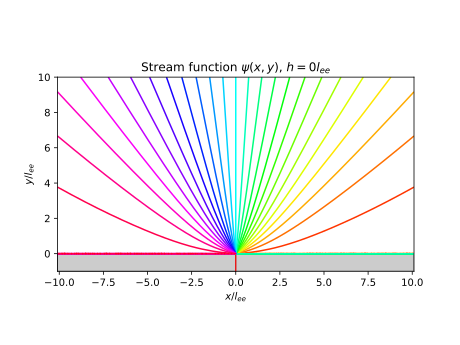
\includegraphics[width=0.4\textwidth]{stream-function-h=0.png}
  \caption{
    \label{fig:edge-stream}
    Stream lines describing current injection by a source placed at
    the origin. Electric current emitted by the source follows the
    contour lines of the stream function~$\psi(x, y)$.
    At distances~$|r| < l_\mathrm{ee}$, the stream lines
    spread isotropically. At large distances, the density of stream
    lines is suppressed near the edge indicating the no-slip behaviour.
    %This indicates no-slip behaviour.
  }
\end{figure}
\begin{figure}[h]
  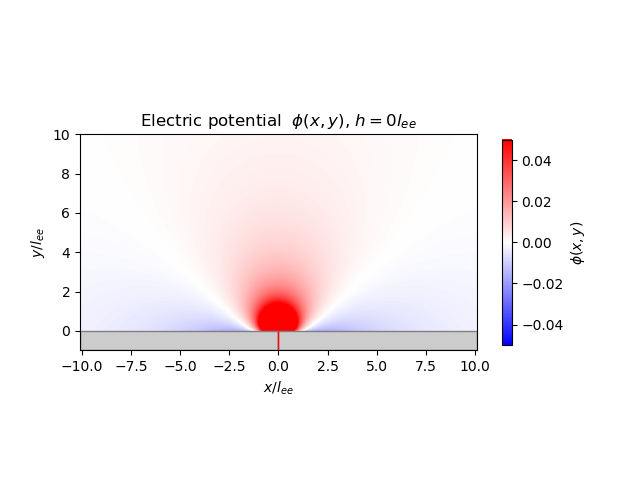
\includegraphics[width=0.6\textwidth]{potential-h=0.png}
  \caption{
    \label{fig:edge-rho}
    Electric potential~$\phi({\bm r})$ induced by the flow shown
    in Fig.~\ref{fig:edge-stream}. While at short distances the behaviour
    is dominated by positive space charge, at larger distances
    the negative potential domain is formed, in agreement with
    fluid mechanics prediction~\cite{bib:Levitov-Falkovich}.
    In an electrically neutral system, the carrier density distribution
    may be converted into the distribution of local eletric
    potential~${\phi}(x, y)$.
  }
\end{figure}
\begin{figure}[h]
  \def\svgwidth{0.5\textwidth}
  \input{flux-h=0.pdf_tex}
  %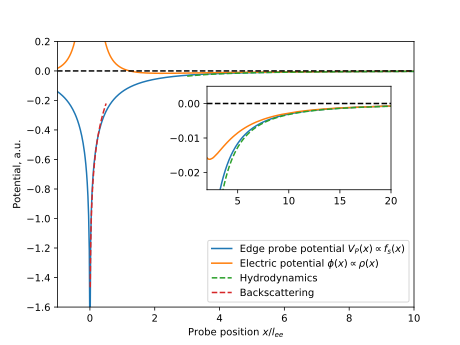
\includegraphics[width=0.4\textwidth]{flux-h=0.png}
  \caption{
    \label{fig:edge-flux}
    The behaviour of both potentials near the source is shown
    as a function of probe position.
    At short distances, the negative signal in~$V_P$ is due to
    the holes backscattered into the edge~\cite{bib:Shytov-et-al}.
    Inset: long-distance behaviour. Local equilibrium is reached,
    the negative flux and density is due to the viscous
    drag~\cite{bib:Levitov-Falkovich}.
  }
\end{figure}
%Another way to probe the crossover is to fabricate probe contacts on
%the edge and pmeasure the vicinity resistance\cite{bib:Bandurin}.
%Such a probe senses the incident flux of particles i.e.
%$V_P \propto f_s(x_P)$, where~$V_P$ is the voltage on the probe,
%and~$x_P$ is the probe position. In a non-equilibrium system,
%it may differ significantly from the local chemical potential
In  Fig.~\ref{fig:edge-flux}, we compare the electric potential~$\phi(x, 0)$
at the edge with with the signal registered by an edge probe,
$V_P(x) \propto f_s(x)$. The two quantities behave very differently
at short distances, $|x| < l_\mathrm{ee}$ which indicates highly
non-equilibrium distribution.
Unlike electric potential, the probe potential is negative even at
the shortest distances~$|x| < l_\mathrm{ee}$ and
does not exhibit space-charge behaviour. This indicates that the
space-charge behaviour is due to charge carriers that  are flying ballistically
parallel to the edge and hence are not caught by the probe.
The singularity~$f_s(x) \propto \log (l_\mathrm{ee}/|x|)$
describes  backscattering of holes into the
probe\cite{bib:Shytov-et-al}, while the behaviour
at large distances shown in the inset to Fig.~\ref{fig:edge-flux}
is described by fluid mechanics.
\begin{figure}[h]
 \def\svgwidth{0.5\textwidth}
  \input{flux-vs-gamma.pdf_tex}
  \caption{
    \label{fig:flux-vs-gamma}
    Dependence of the edge probe potential~$V_P(x_P)$
    on the relaxation rate~$\gamma$. The minimum of the potential
    separates the two regimes, ballistic and viscous, and hence marks
    the onset of fluidity.
  }
\end{figure}

In practice, edge probe is fabricated at a fixed position~$x_P$,
while~$l_\mathrm{ee}$ can be tuned by changing temperature or
carrier density.
Evolution of the probe potential with changing~$\gamma$
can be obtained from the data shown in Fig.~\ref{fig:edge-flux}
by employing an obvious scaling: $V_P(x) \propto \gamma f_s(\gamma x_P)$.
The result is shown in Fig.~\ref{fig:flux-vs-gamma}.
When~$l_\mathrm{ee} < x_P$,
one can observe a negative ballistic signal due to hole backscattering.
The edge potential reaches the deep minimum at~$\gamma x_P \approx 0.79$,
which can be identified as fluidity onset. Indeed, when~$\gamma$ is
increased further, the signal decreases and evolves into the viscous
response.


The~$k = 0$ limit, Eq.~(\ref{eq:fs-k=0}), also provides the solution
to the contact-resistance problem. Let us replace a point source~$I_0$
with  a source equally distributed across the edge,
$I_0(k) \approx \delta(k)$. Current emission results in
an outgoing distribution~$f'(\alpha) \propto 1/\sin\alpha$,
which is partially backscattered into the current-emitting contact.
The limit of~$f_{s, k}$ at~$k = 0$ gives the potential induced by
near the contact and thus represents the contact resistance,
$R_c \approx 1.192$. Restoring  dimensionful units, one can show
that this represents~$1.192$ of Sharvin's conductance, $h/(e^2 k_F W)$,
where~$W$ is the width of the contact, and~$k_F$ is the Fermi momentum.
The contact resistance, however, is not universal:
it strongly depends upon the angular distribution
of emitted particles, and one should repeat the analysis for a different
choice of the source terms~$\dct{\rho}(k, q)$ and~$\dct{\Omega}(k, q)$
o describe contact resistance for a different distribution.

%%%%%%%%%%%%%%%%%%%%%%%%%%%%%%%%%%%%%%%%%%%%%%%%%%%%%%%%%%%%%%%%%%%%%%%%%%%%%
% \begin{figure}                                                            %
%    \subfloat[][]{                                                         %
%      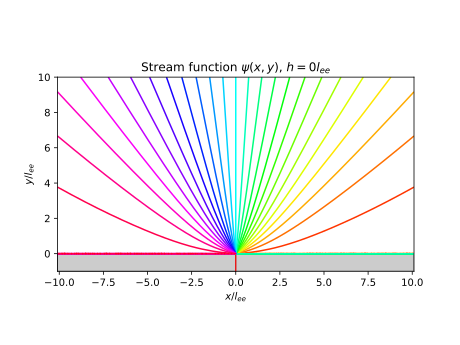
\includegraphics[height=0.25\textwidth]{stream-function-h=0.png}     %
%    }                                                                      %
%    \qquad                                                                 %
%    \subfloat[][]{                                                         %
%       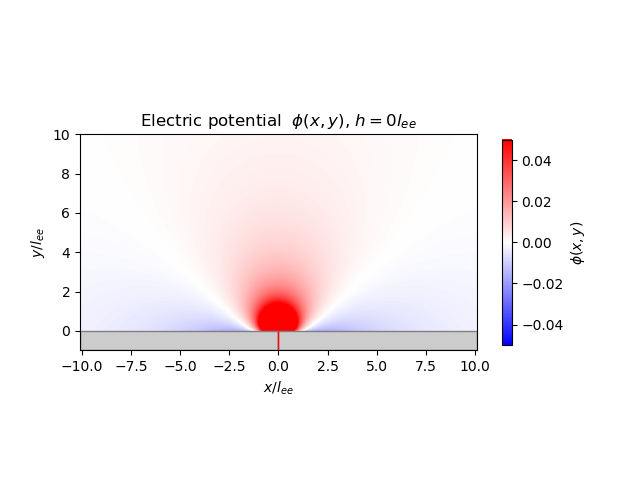
\includegraphics[height=0.3\textwidth]{potential-h=0.png}           %
%     }                                                                     %
%     \caption{                                                             %
%     \label{fig:edge-stream}                                               %
%     (a) Stream lines describing current injection by a source placed at   %
%     the origin. At distances~$|r| < l_\mathrm{ee}$, the stream lines      %
%     spread isotropically. At large distances, the density of stream       %
%     lines is suppressed near the edge.                                    %
%     (b) Carrier density distribution near an injector shown               %
%     in Fig.~\ref{fig:edge-stream}. While at short distances the behaviour %
%     is dominated by positive space charge, at larger distances            %
%     the negative potential domain is formed, in agreement with            %
%     fluid mechanics prediction~\cite{bib:Levitov-Falkovich}.              %
%     In electrically neutral system, the carrier density distribution      %
%     may be converted into the distribution of local eletric               %
%     potential~${\phi}(x, y)$.                                             %
%     }                                                                     %
% \end{figure}                                                              %
%%%%%%%%%%%%%%%%%%%%%%%%%%%%%%%%%%%%%%%%%%%%%%%%%%%%%%%%%%%%%%%%%%%%%%%%%%%%%


\section{Current injection in the interior}
\label{sec:bulk-src}
(ii) Now consider an isotropic current source at $y = h > 0$:
$J(x, y, \alpha) = \delta(x) \delta(y - h) J_0 $,
which in the Fourier representation becomes
$J_{\bm k}(\alpha) = e^{i q h} J_0$.
Applying Eq.(\ref{eq:angular-integrals}), one finds
\begin{equation}
  \label{eq:source-bulk-rho}
  \dct{\rho}^\mathrm{(int)}
  = \frac{J_0 e^{i q h}}{\sqrt{k^2 + q^2 + \gamma^2}}
  = \frac{J_0}{\gamma} \left[1 - K_\rho(k, q) \right]e^{i q h}
  \ ,
\end{equation}
where~$K_\rho(k, q)$ is given by Eq.(\ref{eq:K-rho-def})
The pertinent vorticity contribution vanishes:
$\Omega_\mathrm{direct}^\mathrm{(int)} = 0$.



We can now consider a more difficult problem: a current source placed
in the interior, at~$y = h$. The "direct" contribution to the density is now given
by~$\dct{\rho}(k, q)$, while~$\dct{\Omega}(k, q) = 0$. Hence the solution
for~$\fplusminus{\Omega}_{\bm k}$ can be obtained immediately:
\begin{align}
\Omega_{J, {\bm k}} &=  \fplus{\Omega}(k, q)
= J_\mathrm{ext}^\ast(k) \frac{\fplus{K}_\Omega(k, q)}{K_\Omega^\ast(k)}
= J_0 e^{-|k|h} \frac{\fplus{K}_\Omega(k, q)}{K_\Omega^\ast(k)}
\ ,
\\
\fminus{\Omega}_{\bm k}
&= - J_0 e^{-|k|h} \frac{\fminus{K}_\Omega(k, q)}{K_\Omega^\ast(k)}
\ .
\end{align}
The solution for the density, however, cannot be obtained in an explicit form.
As outlined previously, one has to solve the Riemann-Hilbert problem
\begin{equation}
  \fplus{S}_\rho(k, q) + \fminus{S}_\rho(k, q) = \frac{J_0}{\gamma} e^{iqh}
  \left[\frac{1}{\fminus{K}_\rho(k, q)} -
  \frac{1}{\fplus{K}_\rho(k, q)} \right]
  \ .
\end{equation}
Hence the distortion of the flow due to the wall is described by
\begin{equation}
  \label{eq:bulk-chi-cauchy}
  \fminus{S}_\rho(k, q) = J_0 \int\limits_{-\infty}^{\infty}
  \frac{dq'}{2\pi i} \frac{e^{iq'h}}{\fminus{K}_\rho(k, q') (q - q' - i0)}
  \ .
\end{equation}
The downward flux defined by Eq.(\ref{eq:flux-rho-Omega}) can be related
to the value of~$\fminus{S}_\rho(q = -i|k|)$:
\begin{equation}
  \label{eq:phi-j-prev}
\Phi_J(k) = - \frac{\gamma \gamma' J_0 e^{-|k|h}}{2k^2 \left[K_\rho^\ast(k)\right]^2}
+ \frac{J_0 e^{-|k|h}}{\left[K_\Omega^\ast(k)\right]^2}
+ \frac{\gamma \fminus{S}_\rho(q=-i|k|)}{K_\rho^\ast(k)}
\ .
\end{equation}
The latter can be obtained from the Cauchy integral~(\ref{eq:bulk-chi-cauchy}).
However, fast oscillations in the integrand make the resulting expression
unsuitable for numerical calculations. To resolve this difficulty, one can
transform the integration contour by pulling it to
the upper half-plane~$\Im q > 0$, as shown in Fig.~\ref{fig:contours}.
Interestingly, the pole contribution cancels the first term in Eq.(\ref{eq:phi-j-prev}) in the purely viscous case ($\gamma = \gamma'$).

{\bf ANALYZE/COMMENT on non-cancelling case?}

Hence
\begin{equation}
\Phi_J(k) =
 \frac{J_0 e^{-|k|h}}{\left[K_\Omega^\ast(k)\right]^2}
 + \frac{\gamma J_0}{K_\rho^\ast(k)}
   \int\limits_{\kappa}^{\infty} \frac{ds}{\pi}
   \frac{e^{-hs} \sqrt{s^2 - \kappa^2}}{(s + |k|) (s^2 - k^2) \fplus{K}_\rho(is)}
   \ .
\end{equation}
The secondary source on the boundary is to be found similarly to the previous
section: $f_{s, k} = \pi \Phi_J(k)/\left[1 - \pi \Phi_s(k)\right]$.

As in the previous section, the solution can be employed to obtain current
and potential patterns. Stream function and potential distribution
for~$h/l_\mathrm{ee} = 3$ are shown in Figs.~\ref{fig:bulk-stream}
and~\ref{fig:bulk-rho}, respectively.
The downward flow emitted by the source is transformed
when it hits the edge. This results in an extra broad component of
the potential distribution.
One can see that at sufficiently large distances ($|{\bm r}| > h$) the flow
is similar to the one emitted by a point source on the edge. However,
the sign change in the edge potential occurs at~$x \approx h$
instead of~$l_\mathrm{ee}$.
Evolution of the probe signal with ee relaxation rate is shown in
Fig.~\ref{fig:flux-vs-gamma-h}. In close proximity to the source,
the flux is always positive, fading away into the viscous regime
as~$\propto l_\mathrm{ee}$. Further away, it changes the sign
and exhibits a weaker minimum at the onset of fluidity, $\gamma h \approx 1$.
%In Fig.~\ref{fig:bulk-flux} we show how the
%flux into the wall changes when the electron-electron relaxation length
%is changed: decreasing~$l_\mathrm{ee}$ results in suppression
%of the probe signal. The edge
%signal is minimal when~$x \approx l_\mathrm{ee}$ i.e. at the
%fluidity onset.
\begin{figure}
  \def\svgwidth{0.5\textwidth}
  \input{stream-function-h=3.pdf_tex}
  %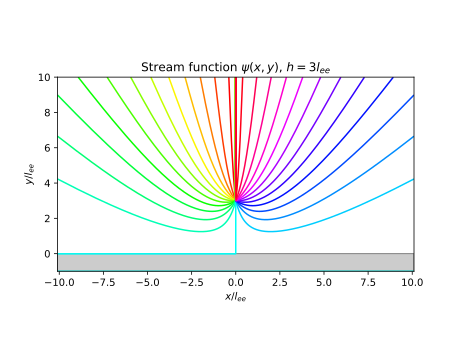
\includegraphics[width=0.4\textwidth]{stream-function-h=3.png}
  \caption{
    \label{fig:bulk-stream}
    Stream function for a flow induced by current injector
     placed~$3l_\mathrm{ee}$ away from the edge.
  }
\end{figure}
\begin{figure}
  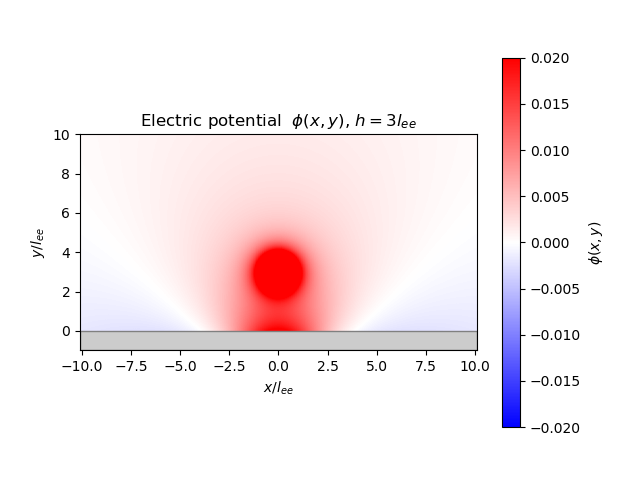
\includegraphics[width=0.6\textwidth]{potential-h=3.png}
  \caption{
    \label{fig:bulk-rho}
    Electric  potential distribution induced by a current injector
    placed~$3l_\mathrm{ee}$ away from the edge.
  }
\end{figure}
\begin{figure}
  \def\svgwidth{0.5\textwidth}
  \input{flux-vs-gamma-h.pdf_tex}
  \caption{
    \label{fig:flux-vs-gamma-h}
    Evolution of edge probe signal with increasing relaxation rate~$\gamma$.
  }
\end{figure}
%\begin{figure}
%  \def\svgwidth{0.5\textwidth}
%  \input{flux-vs-lee.pdf_tex}
%  %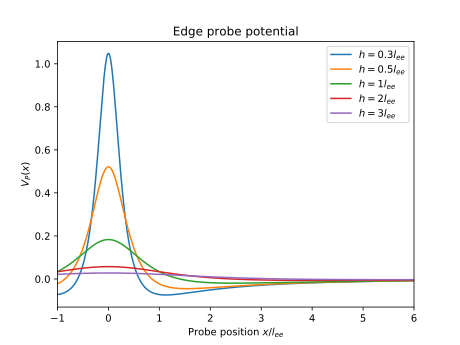
\includegraphics[width=0.5\textwidth]{flux-vs-h.png}
%  \caption{
%    \label{fig:bulk-flux}
%    Edge probe potential for different values of electron mean
%    free path~$l_\mathrm{ee}$.
%  }
%\end{figure}



\section{Momentum source in the interior}
\label{sec:stokeslet}

{\bf STOPPED HERE}
(iii) A point momentum source is described by
\begin{equation}
  \label{eq:source-force-J}
  J^\mathrm{(force)}(x, y, \alpha)
  = 2 (F_x \cos\alpha + F_y \sin\alpha) \delta(x) \delta(y - h)
\ ,
\end{equation}
where~$F_{x, y}$ are the components of the force applied at~$(0, h)$.
A straightforward application of Eq.~(\ref{eq:angular-integrals}) yields
\begin{equation}
  \label{eq:source-force-rho}
  \dct{\rho}^\mathrm{(force)}(k, q)
      =  i \frac{2(k F_x + q F_y)}{k^2 + q^2}
               K_\rho(k, q)  e^{i q h}\ ,
\end{equation}
\begin{equation}
  \label{eq:source-force-omega}
  \dct{\Omega}^\mathrm{(force)} = \frac{kF_y - q F_x}{\gamma}
                                    \left[1 - K_\Omega(k, q)\right] e^{i q h}
  \ .
\end{equation}

This problem is defined by Eqs.(\ref{eq:source-force-rho})
and~(\ref{eq:source-force-omega}). Since the source does not inject particles,
~$\fplus{D}(k, q) = 0$. Comparing this with the previous problem,
one can notice certain duality: the density and vorticity interchange their
roles. The density can be found straightforwardly via elimination of the pole
at~$q = i|k|$:
\begin{align}
  \rho_F(k, q) &\equiv \fplus{\rho}(k, q) = \frac{2i(k F_x + q F_y)}{k^2 + q^2}
  e^{iqh} - \frac{i\sgn k F_x - F_y}{|k| + i q}
   \frac{\fplus{K}_\rho(k, q)}{K_\rho^\ast(k)} e^{-|k|h}
  \ ,
  \\
  \fminus{\rho}(k, q) &= \frac{i\sgn k F_x - F_y}{|k| + iq}
   \frac{\fminus{K}_\rho(k, q)}{K_\rho^\ast(k)} e^{-|k|h}
  \ .
\end{align}
The correction to the vorticity~$\fminus{S}_\Omega$ can be found
 by solving the Riemann-Hilbert problem
\begin{equation}
  \fplus{S}_\Omega(k, q) + \fminus{S}_\Omega(k, q) =
  \frac{k F_y - qF_x}{\gamma} e^{iqh} \left[\frac{1}{\fminus{K}_\Omega(k, q)}
   - \frac{1}{\fplus{K}_\Omega(k, q)} \right]
  \ .
\end{equation}
 As usual, the solution is given
by the Cauchy integral~(\ref{eq:solution-psi}):
\begin{equation}
  \fminus{S}_\Omega(k, q) + S_\Omega^\ast(k) =  \int\limits_{-\infty}^{\infty}
  \frac{dq'}{2\pi i}
  \frac{(i|k| - q) e^{iq'h}}{(q - q' - i0)(i|k| - q' - i0)}
  \frac{k F_y - q'F_x}{\gamma}
  \left[\frac{1}{\fminus{K}_\Omega(k, q')}
            - \frac{1}{\fplus{K}_\Omega(k, q')}\right]
  \ .
\end{equation}
In this integral, the contour can be also transformed into a contribution of
the pole at~$q' = i |k|$ and the branch cut, as shown in Fig.~\ref{fig:contours}.
Evaluating the flux as usual, we write
\begin{equation}
  \Phi_F(k) = \frac{\gamma}{2|k|}\frac{i F_x \sgn k - F_y}{\left[K_\rho^\ast(k)\right]^2}
  e^{-|k| h} - \frac{1}{K_\Omega^\ast(k)} \left[\fminus{S}_\Omega(k, -i|k|) + S_\Omega^\ast(k)\right]
  \ .
\end{equation}
This expression can be rewritten as
\begin{equation}
  \Phi_F(k) =  (i F_x \sgn k - F_y)e^{-|k|h}
  \left[\frac{\gamma}{2|k|\left[K_\rho^\ast(k)\right]^2} - \frac{|k|}{\gamma\left[K_\Omega^\ast(k)\right]^2 }\right]
  -  \frac{|k|}{\gamma}\int\limits_C \frac{dq'}{\pi} \frac{e^{iq'h}}{q'^2 + k^2}
     \frac{k F_y - q'F_x}{\fminus{K}_\Omega(k, q')}
     \ .
\end{equation}
As before,~$f_s(k)$ is obtained from flux conservation condition,
$f_s(k) = \pi \Phi_F(k)/(1 - \pi \Phi_s(k))$.

The stream pattern and the potential induced by a point momentum
source acting in the $x$-direction (parallel to the edge)
are shown in Figs.~\ref{fig:cos-stream} and~\ref{fig:cos-rho}
for~$h = 3l_\mathrm{ee}$. The flow and the potential for a source acting
along the $y$ axis are showin in Figs.\ref{fig:sin-stream}
and~\ref{fig:sin-rho}. The two stream patterns are affected by
the edge even though the distance to the edge exceeds the mean free path.
This can be seen e.g. by noting that \ref{fig:cos-stream}
cannot be obtained from Fig.\ref{fig:sin-stream} via a $90^\circ$
rotation, as one would expect in an infinite system.
To resolve this paradox, one can first calculate the Stokeslet in an infinite
space starting either from the Stokes equation, or from the Boltzmann
equation and taking the limit~$|{\bm k}| \ll \gamma$. This way, one can
identify a logarithmic infrared divergence in the current distribution.
This divergence indicates that in two dimensions the Stokeslet cannot
be properly defined without considering the effect of boundary conditions
irrespective of the distance to the edge. The boundary condition regularises
the log-divergence differently for two different orientation of the momentum
source, and this is seen as the difference between
Figs.~\ref{fig:cos-stream} and~\ref{fig:sin-stream}.
%This reflects momentum conservation in electron-electron collisions.
%Indeed, in an infinite space one can identify

%One can also see how the momentum source affects voltage on a probe attached
%to the edge.
This physics, however, is not seen  in the
edge probe potentials
%induced by $x$- and $y$-momentum sources are
shown in Figs.~\ref{fig:cos-flux} and~\ref{fig:sin-flux}
respectively for different values of electron-electron
mean-free path~$l_\mathrm{ee}$.
One can see that the edge potential dependence on~$l_\mathrm{ee}$ is
very weak.
%This can be understood by inspecting the Stokeslet in
%an infinite space.
To explain this, note that the Stokeslet in an infinite space is
characterised by pressure  response
by~$p({\bm r}) = {\bm F} \cdot{\bm r}{r^2}$, where~${\bm F}$ is the
force applied at the origin. This relation holds irrespective
of the relationship between~$|{\bm r}|$ and~$l_\mathrm{ee}$.
Apparently, edge potentials shown in  Figs.~\ref{fig:cos-flux}
and~\ref{fig:sin-flux} receive the dominant contribution from this
longitudinal mode.
%One can see that the
%potential is strong at~$h \ll l_\mathrm{ee}$, becomes suppressed
%when~$h \sim l_\mathrm{ee}$, however, it
%decays rather slowly when~$h > l_\mathrm{ee}$.

Experimentally, point momentum source can be realised in scanning microscopy
experiments in which the scanning gate depletes the system and thus blocks
the passage of current~\cite{bib:Ensslin}. A simple model for this is a
perturbation of a flow by a pointlike scatterer. Introducing the scatterer
to the right-hand side of Boltzmann's equation, one can see that it effectively
acts as a source of momentum and higher angular harmonics of the distribution
function. (Emission of the density harmonic is suppressed by particle number
conservation.) At large distances, the effect of the scatterer is dominated by the lowest harmonic, i.e. by $x$- and $y$-components of momentum.

\begin{figure}
  \def\svgwidth{0.5\textwidth}
  \input{stream-function-h=3-cos.pdf_tex}
  %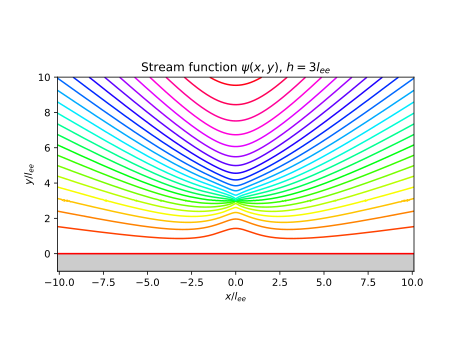
\includegraphics[width=0.4\textwidth]{stream-function-h=3-cos.png}
  \caption{
    \label{fig:cos-stream}
    Stream function for a flow induced by a point momentum source
    acting parallel to the wall and placed at~$(0, 3l_\mathrm{ee})$.
  }
\end{figure}
\begin{figure}
  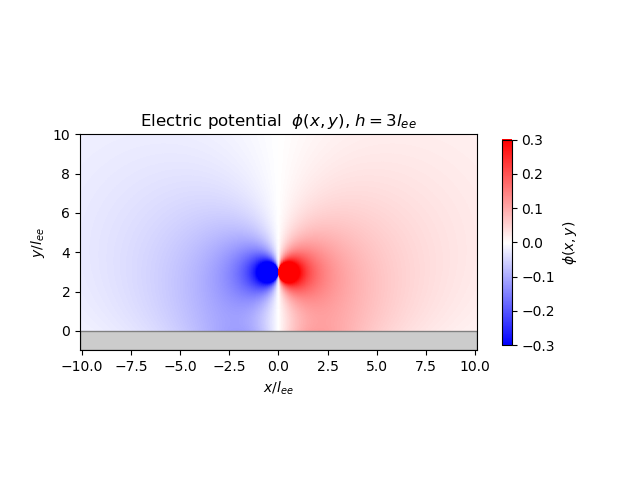
\includegraphics[width=0.6\textwidth]{potential-h=3-cos.png}
  \caption{
    \label{fig:cos-rho}
    Potential distribution for the flow shown in Fig.~\ref{fig:cos-stream}.
  }
\end{figure}
\begin{figure}
  \def\svgwidth{0.5\textwidth}
  \input{stream-function-h=3-sin.pdf_tex}
  %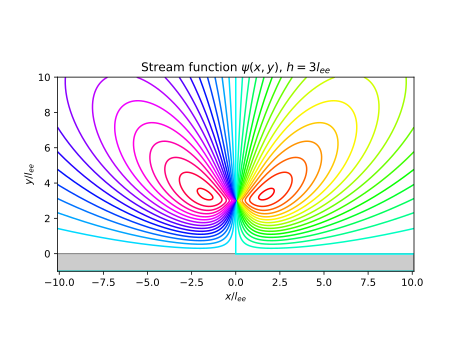
\includegraphics[width=0.4\textwidth]{stream-function-h=3-sin.svg}
  \caption{
    \label{fig:sin-stream}
    Stream function for a flow induced by a point momentum source
    acting perpendicular to the wall and placed at~$(0, 3l_\mathrm{ee})$.
  }
\end{figure}
\begin{figure}
  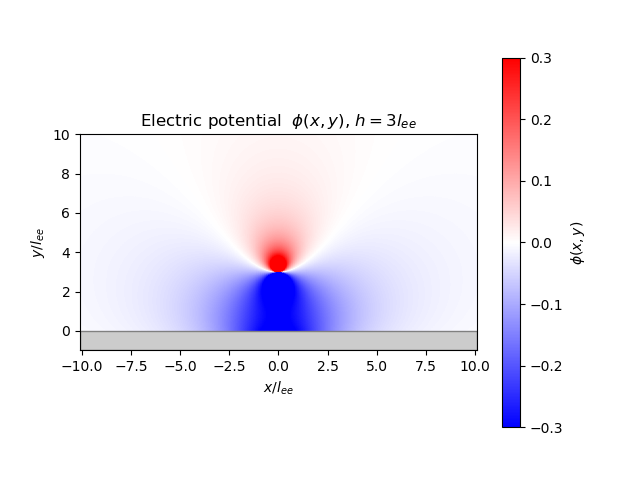
\includegraphics[width=0.4\textwidth]{potential-h=3-sin.png}
  \caption{
    \label{fig:sin-rho}
    Potential distribution for the flow shown in Fig.~\ref{fig:sin-stream}.
  }
\end{figure}

\begin{figure}
  \def\svgwidth{0.5\textwidth}
  \input{flux-vs-lee-cos.pdf_tex}
  %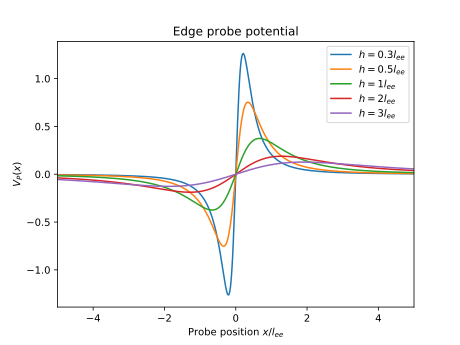
\includegraphics[width=0.4\textwidth]{flux-vs-h-cos.png}
  \caption{
    \label{fig:cos-flux}
    The potential induced at the edge by a flow shown in Fig.~\ref{fig:cos-stream}.
  }
\end{figure}
\begin{figure}
  \def\svgwidth{0.5\textwidth}
  \input{flux-vs-lee-sin.pdf_tex}
  %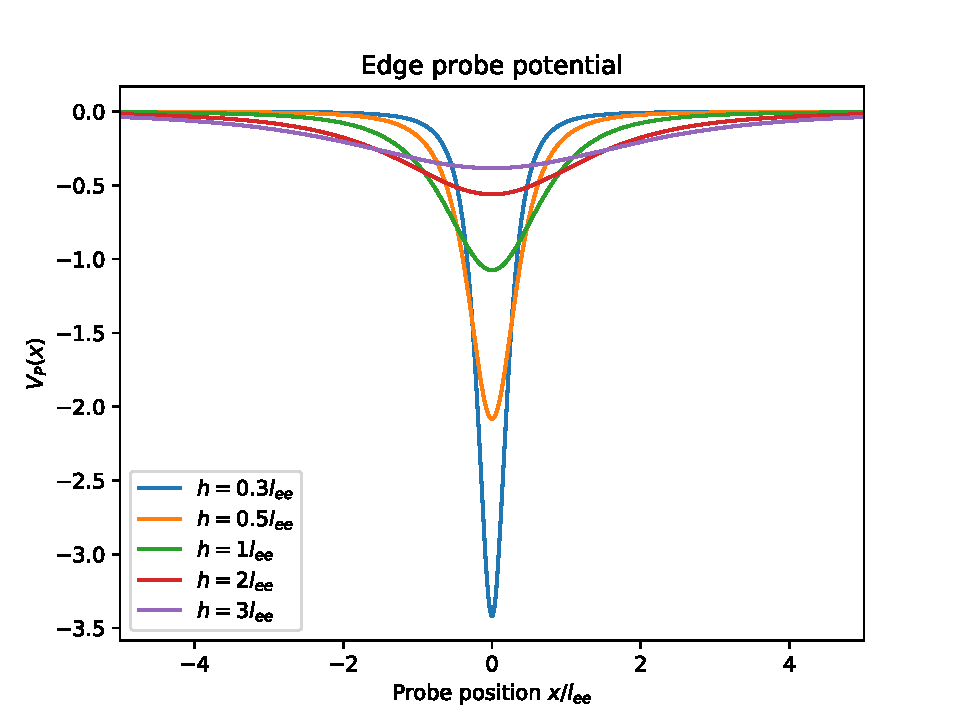
\includegraphics[width=0.4\textwidth]{flux-vs-h-sin.png}
  \caption{
    \label{fig:sin-flux}
    The potential induced at the edge by a flow shown in Fig.~\ref{fig:sin-stream}.
  }
\end{figure}

Our solution can be also employed to extract the slip length~$\lambda$.
To this end, consider the limit of uniform flow, $k = 0$,
in which the source of $x$-momentum is distributed over
the interior, e.g. $F_x(y) = F_0 \exp(-\delta y)$, where~$\delta \ll y$.
Such a force induces a Poiseuille-like flow in which the role of
the channel width~$W$ is played by~$\delta^{-1}$. The equation for
vorticity,
\begin{equation}
  K_\Omega(0, q) \fplus{\Omega}_q + \fminus{\Omega}_q =
  - \frac{q F_0}{2\gamma (\delta - i q)} \left[1 - K_\Omega(0, q)\right]
  \ ,
\end{equation}
is readily solved by dividing both sides by~$\fminus{K}_\Omega(0, q)$,
separating the pole at~$q = -i \delta$ from~$\fminus{\Omega}$,
and using the consistency condition~$\fplus{\Omega}(0, 0) = 0$. This yields
\begin{equation}
  \fplus{\Omega}_q = \frac{F_0}{2\gamma} \frac{q}{\delta - i q}
  \left[1 - \frac{\fplus{K}_\Omega(0, q)}{\fminus{K}_\Omega(0, -i \delta)}
  \right]
  \ .
\end{equation}
By definition,
the slip length is obtained by extrapolating current profile
at~$y \gg \gamma^{-1}$ to~$y = 0$.
Hence we consider the current density~$j_x(y)$
at~$\gamma^{-1} \ll y \ll \delta^{-1}$, i.e. at~$\delta \ll q  \ll \gamma$.
Employing the results of Appendix~\ref{sec:k=0-limit}
\begin{equation}
  \fplus{K}_\Omega(0, q\ll \gamma) \approx \frac{2\gamma}{-iq} + \frac{4}{\pi}
  \ ,
\end{equation}
one finds the two leading terms:
\begin{equation}
  j_x(q) = - \frac{\fplus{\Omega}_q}{q} = - \frac{2 \gamma F_0}{q^2\delta}
  + \frac{4}{(-iq)  \pi \delta}
  \ .
\end{equation}
In real space, the first term represents a uniform velocity shear near the
edge, $j_x^{(1)}(y) = 2 \gamma F_0 \delta^{-1} y$, while the second term
adds a constant offset: $j_x^{(2)} = 4 / \pi \delta^{-1}$. The slip
length is therefore given
by~$\lambda = 2/(\pi \gamma) \approx 0.64 \gamma^{-1}$.

It is interesting to compare this result with the result for~$f_s(k)$
due to a point source. Solving hydrodynamical equations with a finite
slip length~$\lambda$, one finds for Fourier components of
pressure at the edge:
$p_k \propto |k| (1 + \lambda |k|)/(1 + 2 \lambda|k|)
\approx |k| - \lambda |k|^2$. Naively, one should expect the
density at the edge~$f_s(k)$ to be proportional to pressure.
Using our result for~$\lambda$, one
finds the quadratic term to be~$-0.64 |k|^2/\gamma$. This is close
to our previous result, Eq.(\ref{eq:fs-k=0}), in which the relevant
coefficient is~$-0.707$. The difference is due to the variation
of the density near the edge at distances~$y\sim\gamma^{-1}$.

\section{Conclusion}
\label{sec:conclusion}



Analytical treatment of fluidity onset in this article can be employed
to provide detailed answers to many questions, to make connections with
experiments, and perhaps to develop approximate schemes for many
interesting setups which are not covered here.
For example, one can also incorporate Drude momentum relaxation into
the Wiener-Hopf approach by modifying the kernels~$K_\rho(k, q)$
and~$K_\Omega(k, q)$. Another  interesting open questions is whether it is
possible to incorporate (weak) external magnetic field into the formalism,
which is important for a number of interesting measurements.

The solution, besides being fully quantitative, provides some interesting
insights. For example, the ability to represent the solution in terms of
pole and cut contribution describes a separation between degrees of freedom
which can be helpful for qualitative analysis.

to be continued.



\appendix

\section{Treating one-sided boundary sources}
\label{sec:sources}
%Here we shall consider the following four
%types of external sources: (i) an isotropic current source at the interface,
%$y = 0$, (ii) an isotropic current source in the interior,
%(iii) a point momentum source in the interior (Stokeslet),
%(iv) the Lambertian source representing diffuse scattering at the edge.

%Before attempting a solution of the Wiener-Hopf equations, let us discuss
%the actual form of the sources.
%As we will see below,
%in many important cases solving the Wiener-Hopf equations can be facilitated
%due to a particular form of the source terms.

In this appendix, we show how one can treat boundary sources,
i.e., an isotropic emitter and a Lambertian diffuse source, without extending
them to the lower semispace.

Let us begin with the emitter described by the source term
$J^{\mathrm{edge}}(x, y, \alpha) = 2 I_0 \delta(x)\delta(y) \Theta(\alpha)$,
where~$I_0$ is the total current injected by the source. In the Fourier
representation, this becomes~$J_{\bm k}(\alpha) = I_0 \Theta(\alpha) / \pi$.
The respective direct-flight contribution to the density reads
\begin{equation}
   \label{eq:source-surf-rho-app}
  \dct{\rho}^{\mathrm{(edge)}}(k, q)
  = \int\limits_{0}^{\pi}
         \frac{d\alpha}{2\pi} \frac{J_{\bm k}(\alpha)}{\gamma
                               - i {\bm k} \cdot {\bm v}} = 2 I_0 F_m(k, q) \ .
\end{equation}
The quantity
\begin{equation}
F_m(k, q) \equiv \int\limits_{0}^{\pi}  \frac{d\alpha}{2\pi}
               \frac{1}{\gamma - i k \cos \alpha - i q \sin\alpha}
\end{equation}
represents the ``master integral'' through which we shall express
all other contributions of ``one-sided'' sources.
A straightforward calculation (e.g. by changing the
integration variable to~$z = e^{i\alpha}$) yields
\begin{equation}
  \label{eq:source-fm-def}
  F_m(k, q) = \frac{1}{2\sqrt{k^2 + q^2 + \gamma^2}}
  \left[1 + \frac{2i}{\pi}
               \log\frac{q + \sqrt{q^2 + k^2 + \gamma^2}}{\sqrt{k^2 + \gamma^2}}\right]
\end{equation}
(the logarithm in the brackets can be also written
as~$\sinh^{-1} (q / \sqrt{k^2 + \gamma^2})$). By definition, this function
is complex-analytic at~$\Im q > 0$, as all poles in the integrand are
at~$\Im q < 0$ for upward-going particles. The function~$F_m(k, q)$
satisfies the identity
\begin{align}
  \label{eq:fm-identity}
  F_m(k, q) + F_m(k, -q) = \frac{1 - K_\rho(k, q)}{\gamma} \ ,
  %\qquad
\end{align}
in which the right-hand side describes a fully isotropic current source, 
cf. Eq.(\ref{eq:I-src-rho-omega}), while the two terms on the
left-hand side describe upward-going and downward-going particles.
The function~$F_m(k, -q)$ is complex-analytic in the lower half-plane.
%It can be also represented as the
%Fourier image of the density induced by a point source via "direct flights",
%$|{\bm r}|^{-1} \exp (-\gamma |{\bm r}|)$,
%restricted to the half-space~$y > 0$.)
% induced by the source via "direct flight",
% restricted to the semispace~$y > 0$.
The direct-flight contribution to the vorticity is also straightforward,
and one arrives at a  $q$-indepdendent expression:
\begin{equation}
  \label{eq:source-surf-omega-app}
  \dct{\Omega}^{\mathrm{(edge)}}(k, q) =
  \int\limits_{0}^{\pi} \frac{d\alpha}{2\pi} \frac{J_{\bm k}(\alpha)
        ({\bm k} \times {\bm v})}{\gamma - i {\bm k} \cdot {\bm v}}
    = \frac{2 I_0}{\pi} \tan^{-1} \frac{k}{\gamma}\ .
\end{equation}

Now we can solve the Wiener-Hopf equations with these sources.
To decompose the source in the density equation
%\begin{align}
%S_\rho(k, q) = 2I_0 \frac{F_m(k, q)}{\fminus{K}_\rho(k, q)}
%\end{align}
into  $\fplusminus{S}_\rho(k, q)$, we
apply the identity~(\ref{eq:fm-identity}):
\begin{equation}
  \fplus{S}_\rho(k,q) + \fminus{S}_\rho(k, q)
  = \frac{2 I_0 F_m(k, q)}{\fminus{K}_\rho(k, q)}
= \frac{2I_0}{\gamma}
\left[ -  \frac{\gamma F_m(k, -q)}{\fminus{K}_\rho(k, q)}
+ \frac{1}{\fminus{K}_\rho(k, q)}  -  \frac{1}{\fplus{K}_\rho(k, q)}\right]
\  .
\end{equation}
Since the function~$F_m(k, -q)$ is analytic at~$\Im q < 0$,
the first two terms can be grouped into~$\fminus{S}_\rho(k, q)$.
Hence we find the solution decaying at~$q\to \infty$:
\begin{equation}
\fminus{S}_\rho(k, q) = \frac{2I_0}{\gamma}
\left[ - \frac{\gamma F_m(k, -q)}{\fminus{K}_\rho(k, q)}
       + \frac{1}{\fminus{K}_\rho(k, q)} - 1
\right]
\ ,
\end{equation}
while~$\fplus{S}_\rho(k, q)$ is the same as in Eq.~(\ref{eq:iso-chi}),
so that only the density~$\fminus{\rho}(k, q)$ is changed by
$\Delta\fminus{\rho}(k, q) = - I_0 F_m(k, -q)$.
Since the vorticity contribution given by Eq.(\ref{eq:source-surf-omega-app})
is $q$-independent, we can also absorb this constant by
shifting~$\fminus{\Omega}(k, q)$ without changing~$\fplus{\Omega}(k, q)$.
%Handling the vorticity contribution is similar: the
%respective constant term on the right-hand side can be
%absorbed into~$\fminus{\Omega}(k, q)$ by adding an extra contribution
%\begin{equation}
%  \Delta\fminus{S}_\Omega(k, q) = \frac{2}{\pi \fminus{K}_\Omega(k, q)}
%  \tan^{-1}\frac{k}{\gamma}\ .
%\ .
%\end{equation}
%Again, this does not affect~$\fplus{\Omega}(k, q)$.
Thus, the only change occurs in the expression for the downward-going
flux, see Eq.~(\ref{eq:flux-rho-Omega}):
\begin{align}
\Delta \Phi(k) = \gamma \Delta \fminus{\rho}(k, -i|k|) -
\sgn k\, \fminus{\Omega}(k, -i|k)
= I_0 \left[-F_m(k, i|k|) + \frac{2}{\pi} \tan^{-1}\frac{|k|}{\gamma}\right]
\ .
\end{align}
With the help of Eq.~(\ref{eq:source-fm-def}), this simplifies to
$\Delta \Phi(k) = -I_0 / \gamma$, which coincides with the extra flux
employed in Eqs.(\ref{eq:iso-flux-dPhi}) and~(\ref{eq:phi-iso-surf}).

%Using Eq.(\ref{eq:solution-rho-plus}) and~(\ref{eq:solution-omega-plus}),
%we obtain final expressions for
%the density and vorticity induced by the current source alone:
%\begin{align}
%  \label{eq:rho-I}
%\rho_{I, {\bm k}} = \fplus{\rho}_{\bm k}
%&= \frac{2 I_0}{\gamma}\left[\frac{1}{\fplus{K}_\rho(k, q)} - 1\right]
%+ \frac{2 \gamma' I_0}{k^2 + q^2}
%  - \frac{\gamma' I_0}{|k|(|k| + iq)} \frac{\fplus{K}_\rho(k, %q)}{K_\rho^\ast(k)}
%  \ ,
%  \\
%  \label{eq:omega-I}
%\Omega_{I, {\bm k}} = \fplus{\Omega}_{\bm k}
%&= I_0 \frac{\fplus{K}_\Omega(k, q)}{K_\Omega^\ast(k)}  \sgn{k} \ .
%\end{align}

Let us now perform the same analysis for a diffuse source
$J(x, y, \alpha) = f_s(x) \sin\alpha \delta(y)$ restricted to
upward movers. The source in the density equation
\begin{equation}
  \label{eq:source-diff-rho}
  \dct{\rho}^\mathrm{(diff)}(k, q) = f_{s}(k) F_\rho(k, q)
  \ ,
\end{equation}
can be expressed via the master integral:
\begin{equation}
  \label{eq:source-frho-def}
  F_\rho(k, q) \equiv
  \int\limits_{0}^{\pi} \frac{\sin\alpha}{\gamma -
    i k \cos\alpha - i q \sin\alpha}
             \frac{d\alpha}{2\pi}
  =  \frac{1}{k^2 + q^2} \left[ \frac{k}{\pi} \tan^{-1}\frac{k}{\gamma}
                              + \frac{iq}{2}
  - i \gamma q F_m(k, q) \right]
  \ .
\end{equation}
It obeys an identity similar to Eq.~(\ref{eq:fm-identity}):
\begin{align}
\label{eq:frho-identity}
F_\rho(k, q) &-  F_\rho(k, -q) = \frac{i q}{q^2 + k^2} K_\rho(k, q)
\ ,
\end{align}
where again the right-hand side represents a source extended to
the whole unit circle, cf. Eq.~(\ref{eq:phi-s-low}),
which is decomposed into upward- and downward
movers. The function~$F_\rho(k, q)$ is analytic in the upper half-plane,
while the function~$F_\rho(k, -q)$ is analytic in the lower half-plane.
The respective vorticity contribution
$ \dct{\Omega}^\mathrm{(diff)}(k, q) = f_{s}(k) F_\Omega (k, q) $,
%\begin{equation}
%\end{equation}
is again expressed via the master integral:
\begin{align}
%\label{eq:source-fomega-def}
\label{eq:source-diff-omega}
  F_\Omega(k, q) \equiv{}&  \int\limits_{0}^{\pi}
              \frac{\sin\alpha (k \sin \alpha - q \cos\alpha)}{\gamma
                - i k \cos\alpha - i q \sin\alpha} \frac{d\alpha}{2\pi} && &
  \\
  ={}& k \left(1 + \frac{\gamma^2}{k^2 + q^2}\right) F_m(k, q)
                 -\frac{1}{2} \frac{\gamma k}{k^2 + q^2}
  - \frac{i}{\pi} \frac{\gamma q}{k^2 + q^2} \tan^{-1}\frac{k}{\gamma}
  \ .
  \nonumber
\end{align}
The function~$F_\Omega(k, q)$ obeys the identity
\begin{align}
\label{eq:fomega-identity}
F_\Omega(k, q) & + F_\Omega(k, -q)
        = \frac{k}{2\gamma} \left[1 - K_\Omega(k, q)\right]
\ ,
\end{align}
which has the same interpretation as Eqs.(\ref{eq:fm-identity})
and~(\ref{eq:frho-identity}), with the right-hand side
matching Eq.(\ref{eq:phi-s-low}).
The Wiender-Hopf equations are solved in the same manner as before.
The function~$\fminus{\rho}(k, q)$ acquires an extra contribution
$\Delta \fminus{\rho}(k, q) = f_s F_\rho(k, -q)$, while
the function~$\fplus{\rho}(k, q)$ is again determined 
by Eq.~(\ref{eq:rho-s}). Similarly, $\fplus{\Omega}(k, q)$
remains the same as in Eq.(\ref{eq:omega-s}),
while $\fminus{\Omega}(k, q)$
is shifted by~$\Delta\fminus{\Omega}(k, q) = - f_s F_\Omega(k, -q)$.
The respective change in flux is given by
\begin{align}
\Delta \Phi(k)
= f_s(k) \left[F_\rho(k, i|k|) + \sgn k F_\Omega(k, i|k|)\right]
\ .
\end{align}
Using Eqs.(\ref{eq:source-frho-def})
and(\ref{eq:source-diff-omega}),
this expression simplifies to~$f_s(k) / \pi$. 



%The following facts facilitate solving the Wiener-Hopf equations.
%First, note that the quantities~$F_m(k, q)$, $F_\rho(k, q)$
%and~$F_\Omega(k, q)$ are
%complex-analytic at~$\Im q > 0$. Hence their mirror images,
%~$\tilde{F}_m \equiv F_m(k, -q)$,
%${\tilde F}_{\rho} \equiv F_\rho(k, -q)$,
%and~$\tilde{F}_\Omega(k, q) \equiv F_\Omega(k, -q)$ are
%complex-analytic at~$\Im q < 0$. It is easy to verify the following relations
%between the functions in each pair:
%\begin{align}
%  \label{eq:fm-identity}
%  F_m(k, q) &+ \tilde{F}_m(k, q) = \frac{1 - K_\rho(k, q)}{\gamma} \ , \\
%  %\qquad
%  \label{eq:frho-identity}
%  F_\rho(k, q) &- \tilde{F}_\rho(k, q) = \frac{i q}{q^2 + k^2} K_\rho(k, q)
%  \ ,\\
%  \label{eq:fomega-identity}
%  F_\Omega(k, q) &+ \tilde{F}_\Omega(k, q)
%          = \frac{k}{2\gamma} \left[1 - K_\Omega(k, q)\right]
%  \ .
%\end{align}

%The solutions involve the values of the functions~$F_m(k, q)$,
%$F_\rho(k, q)$ and~$F_\Omega(k, q)$ at the pole~$q = i |k|$.
%Expanding Eqs.(\ref{eq:source-fm-def}), (\ref{eq:source-frho-def})
%and~(\ref{eq:source-diff-omega}), one finds
%\begin{align}
%  \label{eq:fm-star}
%  F_m^\ast(k) \equiv F_m(k, q = i |k|)
%       ={}& \frac{1}{2\gamma}
%        \left[ 1 - \frac{2}{\pi}\tan^{-1}\frac{|k|}{\gamma} \right] \\
%  \label{eq:frho-star}
%  F_\rho^\ast(k) \equiv F_\rho(k, q = i |k|)
%  ={}&  \frac{1}{2\pi \gamma} + \frac{1}{2\pi |k|} \tan^{-1}\frac{|k|}{\gamma}
%  - \frac{k}{4\gamma^2}
%    \left[1 - \frac{2}{\pi} \tan^{-1} \frac{|k|}{\gamma}\right]
%  \\
%  \label{eq:fomega-star}
%  F_\Omega^\ast(k) \equiv F_\Omega(k, q = i |k|)
%  ={}& \frac{\sgn k}{2\pi} +  \frac{k}{4\gamma}
%       - \frac{k}{2\pi \gamma}  \tan^{-1}\frac{|k|}{\gamma}
%       - \frac{\gamma}{2\pi k}  \tan^{-1}\frac{|k|}{\gamma}
%  \ .
%\end{align}
%It is easy to verify
%the relation~$\gamma F_\rho^\ast(k) + \sgn k F_\Omega^\ast(k) = 1/\pi$,
%which will be important in the analysis of diffuse scattering contribution.

%To obtain the
%functions~$\fplusminus{S}_{\rho}(k, q)$
%and~$\fplusminus{S}_\Omega(k, q)$ defined
%by Eqs.(\ref{eq:chi-def}) and~(\ref{eq:psi-def}), we employ
%the identities (\ref{eq:frho-identity}) and~(\ref{eq:fomega-identity}):
%\begin{align}
%  \fplus{S}_\rho(k, q) + \fminus{S}_\rho(k, q)
%   = \frac{f_{s, k} F_\rho(k, q)}{\fminus{K}_\rho(k, q)}
%  = \frac{f_{s, k}}{\fminus{K}_\rho(k, q)} \left[ \tilde{F}_\rho(k, q)
%      + \frac{iq}{k^2 + q^2} \frac{\fminus{K}_\rho(k, q)}{\fplus{K}_\rho(k, q)}\right]
%  \ ,
%\\
%\fplus{S}_\Omega(k, q) + \fminus{S}_\Omega(k, q)
%= \frac{f_{s, k} F_\Omega(k, q)}{\fminus{K}_\Omega(k, q)}
%= \frac{f_{s, k}}{\fminus{K}_\Omega(k, q)} \left[ - \tilde{F}_\Omega(k, q)
%      + \frac{k}{2\gamma}
%      - \frac{k}{2\gamma}\frac{\fminus{K}_\Omega(k, q)}{\fplus{K}_\Omega(k, q)%}\right]
%\ .
%\end{align}
%Since the functions~$\tilde{F}_\rho(k, q)$ and~$\tilde{F}_\Omega(k, q)$
%are complex-analytic at~$\Im q < 0$, and the remaining terms are analytic
%at~$\Im q > 0$ except the pole at~$q = i |k|$,
%we can find~$\fminus{S}_\rho(k, q)$ and~$\fminus{S}_\Omega(k, q)$ directly:
%\begin{align}
%  \fminus{S}_\rho(k, q) &= f_{s, k} \left[
%  \frac{{F}_\rho(k, -q)}{\fminus{K}_\rho(k, q)}
%  - \frac{1}{2(|k| + iq) K_\rho^\ast(k)}
%  \right]
%  \ ,
%  \\
%  \fminus{S}_\Omega(k, q) + S_\Omega^\ast(k)
%  &= f_{s, k}\left[\frac{k}{2\gamma} \left(\frac{1}{\fminus{K}_\Omega(k, q)}
%  - \frac{1}{K_\Omega^\ast(k)} \right)
%   - \frac{F_\Omega(k, -q)}{\fminus{K}_\Omega(k, q)}  \right]
%%  \ \ ,
%  \\
%%  S_\Omega^\ast(k) &= - \frac{k}{2\gamma} \frac{f_s(k)}{K_\Omega^\ast(k)}
%  \ .
%\end{align}
%We also give explicit expressions for density and vorticity:
%\begin{align}
%  \label{eq:rho-s-app}
%  \rho_{s, {\bm k}} = \fplus{\rho}(k, q) &= f_{s, k} \left[\frac{-iq}{k^2 + q^2}
%  + \frac{1}{2(|k| + iq)} \frac{\fplus{K}_\rho(k, q)}{K_\rho^\ast(k, q)} \right]
%  \\
%   \label{eq:omega-s-app}
%  \Omega_{s, {\bm k}} = \fplus{\Omega}(k, q)
%  &= \frac{k}{2\gamma}
%     \left(\frac{\fplus{K}_\Omega(k, q)}{K_\Omega^\ast} - 1\right)
%  \ .
%\end{align}
%(Note that the diffuse scattering does not contribute to~$\fplus{D}_{\bm k}$,
%according to Eq.(\ref{eq:solution-D}).)


\section{Factorization of the kernels near the poles}

The Wiener-Hopf analysis given in this text often involve the
values of the kernels~$\fplus{K}_\rho(k, q)$ and~$\fplus{K}_\Omega(k, q)$ near
their poles. In this section, we derive the relevant expression
and discuss their long-distance and short-distance behavior.
To this end, we first consider a more general kernel:
\begin{align}
  \mathcal{K}_\alpha(q) = 1 - \frac{\alpha}{\sqrt{q^2 + \kappa^2}}\ .
\end{align}
The kernel~$K_\rho(q)$ is obtained if one takes~$\kappa^2 = k^2 + \gamma^2$
and~$\alpha = \gamma$, while the kernel~$K_\Omega$ is given by
the product of two such kernels:
\begin{align}
  \label{eq:appA-representation}
  K_\rho(k, q) = \mathcal{K}_\gamma(q)\ , \qquad
  K_\Omega(k, q) = \frac{q^2 + \kappa^2}{q^2 + k^2}
 \mathcal{K}_{\gamma}(q) \mathcal{K}_{\gamma' - \gamma''}(q)\ .
\end{align}
The kernel~$\mathcal{K}_\alpha(q)$ has a zero at~$q = i {\tilde \kappa}$,
with~${\tilde \kappa} = \sqrt{\kappa^2 - \alpha^2}$.
Let us consider the kernel~$\fplus{\mathcal{K}}_\alpha$ at the imaginary axis.
The respective Cauchy integral can be transformed as
\begin{align}
  \log \mathcal{K}_{\alpha}(is) = - \frac{1}{2\pi}
  \int\limits_{-\infty}^{\infty}
  \frac{s dq}{s^2 + q^2} \, \log \mathcal{K}_{\alpha}(q)\ .
\end{align}
We are interested in the value of this integral at the point
$s = {\tilde\kappa}$.
This integral is hard to evaluate, so let us consider its derivatives
with respect to~$s$ and~$\alpha$.
The Cauchy integral for the log derivative takes the form
\begin{align}
  \frac{d}{ds} \log \fplus{\mathcal{K}}_{\alpha}(is)
  = -\int\limits_{-\infty}^{\infty} \frac{qdq}{2\pi (q^2 + s^2)}
  \frac{d}{dq} \log \mathcal{K}_\alpha(q)\ ,
\end{align}
which can be expanded as
\begin{align}
  \frac{d}{ds} \log \fplus{\mathcal{K}}_{\alpha}(is)
  = - \frac{\alpha}{2\pi}
  \int\limits_{-\infty}^{\infty}
  \frac{q^2 dq \left[\alpha + \sqrt{q^2 + \kappa^2}\right]}{
     (q^2 + {\tilde \kappa}^2) (q^2 + \kappa^2) (q^2 + s^2)
  }\ .
\end{align}
The first term can be found e.g. by decomposing it
into primitive fractions:
\begin{align}
  -\frac{\alpha^2}{2\pi}\int\limits_{-\infty}^{\infty}
  \frac{q^2 dq}{(q^2 + s^2) (q^2 + \kappa^2)
  (q^2 + {\tilde{\kappa}^2)}} =
  -\frac{\alpha^2}{2(\kappa + s) ({\tilde{\kappa}} + s)
  (\kappa + {\tilde\kappa})}\ . 
\end{align}
The second term can be recast as a difference between
two integrals of a similar structure:
\begin{align}
  -\frac{\alpha}{2\pi(s^2 - \tilde{\kappa}^2)}
  \int\limits_{-\infty}^{\infty}
  \frac{dq}{\sqrt{q^2 + \kappa^2}}
  \left[\frac{s^2}{q^2 + s^2}
  - \frac{\tilde{\kappa}^2}{q^2 + {\tilde\kappa}^2}\right]\ . 
\end{align}
In the first term here, one may change the integration variable
as~$q = s \tan \theta$, and then as~$u = \sin\theta$, which gives
a standard integral:
\begin{align}
  \int\limits_{-\infty}^{\infty} \frac{s^2 dq}{\sqrt{q^2 + \kappa^2} (q^2 + s^2)} =
  \int\limits_{-1}^{1} \frac{sdu}{\sqrt{\kappa^2 - (\kappa^2 - s^2) u^2}}\ . 
\end{align}
Eventually, one finds
\begin{align}
  \frac{d}{ds} \log \fplus{\mathcal{K}}_{\alpha}(is) = 
  -\frac{\kappa - {\tilde{\kappa}}}{2(\kappa + s) ({\tilde{\kappa}} + s)}
  - \frac{\alpha}{2\pi (s^2 -\tilde{\kappa}^2)}
  \left[\frac{s}{\sqrt{\kappa^2 - s^2}} \cos^{-1}\frac{s}{\kappa}
  - \frac{{\tilde{\kappa}}}{\alpha}
  \sin^{-1}\frac{\alpha}{\kappa}\right]
  \ . 
\end{align}
In particular, one finds at the singularity
\begin{align}
  \label{eq:appA-2nd-half}
  \frac{d}{ds} \log \fplus{\mathcal{K}}_{\alpha}(i{\tilde\kappa})
  = - \frac{\kappa - {\tilde{\kappa}}}{4{\tilde \kappa} (\kappa + {\tilde\kappa})}
  - \frac{\kappa^2}{2\pi{\tilde\kappa}^2 \alpha}
  \sin^{-1}\frac{\alpha}{\kappa} + \frac{1}{2\pi\alpha}\ .
\end{align}


...which can be found by first differentiating the expression over~$\alpha$
and then over~$s$ to accomodate for the pole changing its position:
\begin{align}
  \label{eq:appA-two-contribs}
  \frac{d}{d\alpha} [\log \fplus{\mathcal{K}}_\alpha(i{\tilde \kappa})] =
  \frac{d}{d\alpha} \log \fplus{\mathcal{K}}_\alpha(i{\tilde \kappa})
  + \frac{d{\tilde \kappa}}{d\alpha}
  \frac{d}{ds} \log \fplus{\mathcal{K}}_\alpha (i{\tilde \kappa}) \ .
\end{align}
% with respect to~$\alpha$, and evaluate this derivative at~$\tilde{\kappa}$:

The differentiation with respect to~$\alpha$ yields
\begin{align}
  \left.\frac{d}{d\alpha}\log \mathcal{K}_{\alpha}
  \right|_{s = {\tilde\kappa}}
  = \int\limits_{-\infty}^{\infty}
  \frac{{\tilde\kappa} (\alpha + \sqrt{q^2 + \kappa^2})}{
  \left(q^2 + {\tilde \kappa}\right)^2} \frac{dq}{2\pi}
  \ .
\end{align}
The first term yields~$\alpha /(4{\tilde\kappa}^3)$, while in
the second term one can first change the integraion variable
as~$q = {\tilde\kappa}\cos\theta$, and then as~$u = \alpha \sin\theta$.
This yields
\begin{align}
  \left.\frac{d}{d\alpha}\log \mathcal{K}_{\alpha}
  \right|_{s = {\tilde\kappa}}
  = \frac{\alpha}{4{\tilde\kappa}^2} + \frac{1}{\pi\alpha^2 {\tilde\kappa}}
  \int\limits_{0}^{\alpha} \sqrt{\kappa^2 - u^2} du\ .
\end{align}
Computing the remaining standard integral, one evantually finds
\begin{align}
  \label{eq:appA-1st-half}
  \left.\frac{d}{d\alpha}\log \mathcal{K}_{\alpha}
  \right|_{s = {\tilde\kappa}}
  = \frac{\alpha}{4{\tilde\kappa}^2}
  + \frac{\kappa^2}{2\pi\alpha{\tilde\kappa}^2} \sin^{-1}\frac{\alpha}{\kappa}
  + \frac{1}{2\pi{\tilde\kappa}}\ .
\end{align}


Substituting Eqs.(\ref{eq:appA-1st-half}) and~(\ref{eq:appA-2nd-half})
into Eq.~(\ref{eq:appA-two-contribs}) and taking into account
that~$d{\tilde \kappa}{d\alpha} =  - \alpha/{\tilde\kappa}$,
one can obtain the derivative of the value of~$\fplus{\mathcal{K}}_\alpha$
at the moving pole:
\begin{align}
  \frac{d}{d\alpha} [\log \fplus{\mathcal{K}}_\alpha(i{\tilde \kappa})] =
  \frac{\alpha}{2{\tilde\kappa}} \frac{\kappa}{{\tilde\kappa}^2}
  + \frac{\kappa^2}{\pi\alpha{\tilde\kappa}^2} \sin^{-1}\frac{\alpha}{\kappa}
  \ .
\end{align}
Let us integrate this expression with respect to~$\alpha$
from zero to a finite value. (Obviously, the kernel~$\mathcal{K}_\alpha(q)$
degenerates into unity at~$\alpha = 0$.)
The first term is evaluated via elementary methods:
\begin{align}
  \frac{\kappa}{2} \int \frac{\alpha d\alpha}{(\kappa^2 - \alpha^2)
  (\kappa + \sqrt{\kappa^2 - \alpha^2})}
  = \frac{1}{2} \log\frac{\kappa + \sqrt{\kappa^2 - \alpha^2}}{
    \sqrt{\kappa^2 - \alpha^2}}\ .
\end{align}
In the second term, we change the integration variable via
$\alpha = \kappa x / \sqrt{1 + x^2}$,
so that~$\sin^{-1} \alpha/\kappa = \tan^{-1} x$. This yields
\begin{align}
  \frac{\kappa^2}{\pi} \int\limits_{0}^{\alpha}
  \frac{d\alpha}{\alpha{\tilde\kappa}^2} \sin^{-1}\frac{\alpha}{\kappa}
  = \frac{1}{\pi} \int\limits_{0}^{x_\alpha} \frac{dx}{x} \tan^{-1} x\ ,
\end{align}
where~$x_\alpha = \alpha/\sqrt{\kappa^2 - \alpha^2}$.
Thus, we finally obtain the desired expression
\begin{align}
  \log \fplus{\mathcal{K}}_\alpha(i{\tilde \kappa})
  = \frac{1}{2}\log\frac{\kappa + \sqrt{\kappa^2 - \alpha^2}}{
  \sqrt{\kappa^2 - \alpha^2}}
  + \int\limits_{0}^{x_\alpha}\frac{dx}{\pi x} \tan^{-1} x\ .
\end{align}
The remaining integral~$I(x_\alpha)$
can be expressed in terms of the dilogarithm
$\mathop{\mathrm{Li}}_2(x)$. It has an interesting property
\begin{align}
I(x_\alpha) = I(x_\alpha^{-1}) + \frac{1}{2} \log\frac{1}{x_\alpha}\ ,
\end{align}
which can be verified by splitting the integration domain
into two subintervals,~$[0, 1]$ and~$[1, x_\alpha]$ and
then changing the integration variable as~$y = 1/x$ in the
second contribution.

Let us now apply these results to our kernels~$K_\rho(k, q)$
and~$K_\omega(k, q)$. From the representation~(\ref{eq:appA-representation}),
one finds
\begin{align}
  \log K_\rho^\ast(k) =  \frac{1}{2} \log\frac{k + \sqrt{k^2 + \gamma^2}}{2|k|}
  + \frac{1}{\pi}\int\limits_{0}^{\gamma/|k|}
  \frac{dx}{x} \tan^{-1}x
\ ,
\end{align}
and
\begin{align}
  \log K_\Omega^\ast =  \frac{2}{\pi}
  \int\limits_{0}^{x_0} \frac{dx}{x}\tan^{-1}x
\ .
\end{align}

\textbf{INCOMPLETE: not discussed poles away.}

\section{OLD: Factorized kernels near the poles~$q = \pm i|k|$ and~$q = \pm i {\tilde \kappa}$.}
\label{sec:appendix-kstar}
Wiener-Hopf solutions described in this text often include the values of the
factorised kernels~$\fplus{K}_\rho(k, q)$ and~$\fplus{K}_\Omega(k, q)$ near
the points~$q = \pm i|k|$. Here we derive analytic expressions for these kernels
and discuss their behaviour at~$k \ll \gamma$. Let us begin
with~$K_\rho^\ast \equiv \fplus{K}_\rho(q = i|k|)$. The Cauchy
integral~(\ref{eq:factor-cauchy}) takes the form
\begin{equation}
  \log K_\rho^\ast = - \int\limits_{-\infty}^{\infty}\frac{dq}{2\pi} \frac{k}{k^2 + q^2}
  \, \log\left(1 - \frac{\gamma}{\sqrt{k^2 + q^2 + \gamma^2}}\right)
  \ .
\end{equation}
To calculate it, consider its derivative with respect to~$\gamma$:
\begin{equation}
  \frac{\partial}{\partial \gamma} \log K_\rho^\ast
  = \int\limits_{-\infty}^{\infty}
  \frac{\gamma + \sqrt{\gamma^2 + k^2 + q^2}}{(k^2 + q^2)(\gamma^2 + k^2 + q^2)}
  \frac{kdq}{2\pi}
  \ .
\end{equation}
The first integral here is well-known:
\begin{equation}
\int\limits_{-\infty}^{\infty} \frac{k dq}{2\pi} \frac{\gamma}{(q^2 + k^2)(q^2 + k^2 + \gamma^2)}
 = \frac{1}{2} \frac{\gamma}{\sqrt{k^2 + \gamma^2}(|k| + \sqrt{k^2 + \gamma^2})}
 \ ,
\end{equation}
while the other can be found by first changing the integration variable
to~$q = |k|\tan\theta$, and then to~$u = \sin\theta$:
\begin{equation}
  \int\limits_{-\infty}^{\infty} \frac{kdq}{2\pi}
  \frac{1}{(q^2 + k^2)\sqrt{q^2 + k^2 + \gamma^2}}
  = \frac{1}{2\pi}\int\limits_{-1}^{1} \frac{du}{\sqrt{\gamma^2 + k^2 - \gamma^2 u^2}}
   = \frac{1}{\pi\gamma} \tan^{-1}\frac{\gamma}{|k|}
  \ .
\end{equation}
Hence we find
\begin{equation}
  \frac{\partial}{\partial \gamma} \log K_\rho^\ast =
  \frac{\gamma}{2\sqrt{\gamma^2 + k^2}(|k| + \sqrt{k^2 + \gamma^2})}
  + \frac{1}{\pi} \tan^{-1}\frac{\gamma}{|k|}
  \ .
\end{equation}
Integrating over~$\gamma$ and employing the fact that~$K_\rho (\gamma \to 0) = 1$,
we write
\begin{equation}
  \log K_\rho^\ast(k) =  \frac{1}{2} \log\frac{k + \sqrt{k^2 + \gamma^2}}{2|k|}
  + \frac{1}{\pi}\int\limits_{0}^{\gamma/|k|}
  \frac{dx}{x} \tan^{-1}x
\ .
\end{equation}
(The remaining integral can be related to the dilogaritmic
function~$\mathrm{Li}_2(z)$.)
Similar reasoning yields for~$K_\Omega^\ast$:
\begin{equation}
  \log K_\Omega^\ast = \log K_\rho^\ast + \log\frac{2|k|}{|k| + \kappa}
  + I_\Omega \ ,
\end{equation}
with
\begin{equation}
  I_\Omega = - \frac{|k|}{2\pi}\int\limits_{-\infty}^{\infty}
  \frac{dq}{q^2 + k^2}
  \log \left(1 - \frac{\xi \gamma}{\sqrt{k^2 + q^2 + \gamma^2}}\right)
\ .
\end{equation}
Here we introduce~$\xi = (\gamma' - \gamma'')/\gamma$.
The remaining integral can be calculated in a similar fashion. This yields
\begin{equation}
  \log K_\Omega^\ast = \frac{1}{2} \log \frac{2|k|}{|k| + {\tilde \kappa}}
  + \int\limits_{0}^{\gamma/|k|} \frac{dx}{\pi x}
  \left[\tan^{-1}x
    + \frac{1}{\sqrt{x^2 (1 - \xi^2) + 1}}
     \sin^{-1}\frac{\xi x}{\sqrt{1 + x^2}}
  \right]
  \ .
  \label{eq:ko-star-xi}
\end{equation}
For~$\xi = 1$, the second term in the integral is equal to the firs term,
and Eq.(\ref{eq:ko-star-xi}) simplifies to
\begin{equation}
  \log K_\Omega^\ast =
  \int\limits_{0}^{\gamma/|k|} \frac{dx}{\pi x}\tan^{-1}x
\ .
\end{equation}
%One can use this result to estimate
%\begin{equation}
%  \log K_\Omega^\ast =
%  \log\left\{\left[K_\rho^\ast\right]^2 \frac{2|k|}{|k| + \sqrt{k^2 + \gamma^2}%}\right\}
%= \frac{2}{\pi}\int\limits_{0}^{\gamma} \frac{d\gamma}{\gamma} \tan^{-1}\frac{\%gamma}{|k|}
% \ .
%\end{equation}
To analyse the behaviour of these expressions in the long-wavelength limit,
~$k \ll \gamma$,
one can split the integration range into two subintervals,
$[0, |k|]$ and~$[|k|, \gamma]$.
The integral of arctangent can then be transformed by employing
the change of variable~$\gamma = 1/x$.
Hence one can show that at large~$\gamma / |k|$
\begin{equation}
  \int\limits_{0}^{\gamma/|k|} \frac{\tan^{-1}x}{x}\, dx =
  \frac{\pi}{2} \log(x) + \frac{|k|}{\gamma} - \frac{|k|^3}{9\gamma^3} +  O(|k|^5)
\end{equation}
Thus, at~$k \to 0$
\begin{equation}
  \label{eq:krho-k=0}
  \log  K_\rho^\ast(k) = \log\frac{\gamma}{|k|\sqrt{2}}
        + \frac{|k|}{\gamma} \left(\frac{1}{\pi} + \frac{1}{2}\right)
        - \frac{|k|^3}{9\gamma^3} \left(\frac{1}{\pi} + \frac{3}{4}\right)
        + O(|k|^5)
\end{equation}
Analysis of large-distance behaviour~$K_\Omega^\ast$ is cumbersome
in general, but is facilitated
for viscous and Ohmic cases.
In the viscous limit ($\xi = 1$), one finds
\begin{equation}
  \label{eq:komega-k=0}
  \log  K_\Omega^\ast(k) = \log\frac{\gamma}{|k|} + \frac{2|k|}{\pi\gamma}
                           - \frac{2|k|^3}{9\pi\gamma^3}
                         +   O(|k|^5)
\ .
\end{equation}
In the Ohmic limit ($\xi = -1$), $K_\Omega^\ast = 1$.
%For~$\gamma'' \ll \gamma'$,
%one finds, to the lowest order,
%\begin{equation}
%  \log K_\Omega^\ast \approx
%\end{equation}
%At~$k\to 0$, this results in a similar behaviour:
%$K_\Omega^\ast \approx  C_\Omega \gamma / |k|$.
At short distances, $|k| \gg \gamma$, we find
\begin{equation}
  \label{eq:kstar-k=inf}
  K_\rho^\ast \approx 1 + \frac{\gamma}{\pi |k|}
  \ ,
  \qquad
  K_\Omega^\ast \approx 1 + \frac{2\gamma'}{\pi |k|}
  \  .
\end{equation}

Calculations of current distributions involving~$K_\Omega$ often involve
a double pole at~$q = \pm i |k|$ and hence include the logarithmic derivative
of~$K_\Omega$ at this point. This quantity can be found via a similar
calculation applied to the log-derivative of~$K_\Omega$:
\begin{equation}
  K_\Omega' \equiv \frac{d}{ds} \log \fplus{K}_\Omega(is) =
  \int\limits_{-\infty}^{\infty} \frac{dq}{2\pi} \frac{1}{i|k| - q}
   \frac{d}{dq} \log K_\Omega(k, q)
  \ .
\end{equation}
Simplifying the integrand, one finds
\begin{equation}
  K_\Omega' = - \frac{\gamma}{\pi} \int\limits_{-\infty}^{\infty} dq
  \frac{q^2}{(q^2 + k^2)^2\sqrt{k^2 + q^2 + \gamma^2}}
  \ .
\end{equation}
This integral can be also found by changing the integration variable
via~$u = q / \sqrt{k^2 + q^2}$:
\begin{equation}
  K_\Omega' = - \frac{\gamma}{\pi|k|}
  \int\limits_{-1}^{1} \frac{u^2 du}{\sqrt{k^2 + \gamma^2 - \gamma^2 u^2}} =
  \frac{1}{\pi\gamma} \left[
       1
      - \frac{k^2 + \gamma^2}{\gamma|k|} \tan^{-1}\frac{\gamma}{|k|}
    \right]
    \ .
  \end{equation}

\section{The~$k = 0$ limit.}
\label{sec:k=0-limit}

Uniform flows, such as Poiseuille flow, are described by the limit~$k = 0$.
Let us find~$\fplus{K}_\Omega(0, is)$ at small~$s \to 0$. The Cauchy
integral takes the form
\begin{equation}
  \log\fplus{K}_\Omega(is) = - \frac{2}{\pi}\int\limits_{0}^{\infty}
  \frac{s dq}{s^2 + q^2}
  \log\frac{\sqrt{q^2 + \gamma^2} - \gamma}{q}
  \ .
\end{equation}
To calculate the integral retaining the regular part of~$K_\Omega(0, q)$,
we split the integration range into two: $[0, q_0]$ and~$[q_0, \infty]$,
where~$s \ll q_0 \ll \gamma$. For~$q <  q_0$, we can
rewrite the argument of the logarithm as~$|q|/(2\gamma)$. For~$q > q_0$,
$s^2$ in the denominator can be neglected:
\begin{equation}
  \log\fplus{K}_\Omega(is) = - \frac{2}{\pi}
  \int\limits_{0}^{q_0} \frac{s dq}{q^2 + s^2} \log\frac{q}{2\gamma}
  - \frac{2}{\pi} \int\limits_{q_0}^{\infty}
  \frac{s dq}{q^2} \log\frac{\sqrt{q^2 + \gamma^2} - \gamma}{q}
  \ .
\end{equation}
Using the well-known relation\cite{bib:Gradstein}
\begin{equation}
  \int\limits_{0}^{\infty} \frac{dq}{q^2 + a^2} \log\frac{q}{b}
  = \frac{\pi}{2|a|} \log\frac{|a|}{b}
  \ ,
\end{equation}
we find
\begin{equation}
  \log\fplus{K}_\Omega(is) = \log\frac{2\gamma}{q}
  - \frac{2s}{\pi} \int\limits_{q_0}^{\infty}
  \frac{dq}{q^2} \log\frac{2\gamma\left(\sqrt{\gamma^2 + q^2}  - \gamma\right)}{q^2}
  \ .
\end{equation}
The remaining integral can be found via integration by parts,
which gives
\begin{equation}
  \int\limits_{q_0}^{\infty}
  \frac{dq}{q^2} \log\frac{\sqrt{\gamma^2 + q^2}  - \gamma}{2\gamma}
  = \left[-\frac{1}{q}\log\frac{2\gamma \left(\sqrt{q^2 + \gamma^2} - \gamma\right)}{q^2}
  + \frac{1}{q} - \sqrt{\frac{1}{\gamma^2} + \frac{1}{q^2}} \right]_{q_0}^{\infty}
\approx - \frac{1}{\gamma}
\ .
\end{equation}
Hence
\begin{equation}
  \fplus{K}_\Omega(0, is)
  \approx \frac{2\gamma}{s} \exp\left(\frac{2s}{\pi \gamma}\right)
  \approx \frac{2\gamma}{s} + \frac{4}{\pi}
 \ .
\end{equation}

Add: determine rho(y)

\begin{thebibliography}{99}
\bibitem{bib:momentum-relaxation} Ref to collision integral
\bibitem{bib:wiener-hopf} Wiener-Hopf (Noble?)
\bibitem{bib:Reuter-Sondheimer} Reuter-Sondheimer
\bibitem{bib:Shytov-et-al} Shytov et al
\bibitem{bib:Levitov-Falkovich} Levitov-Falkovich
\bibitem{bib:Ilani} Scanning gate measurements: Ilani?
\bibitem{bib:Bandurin} Vicinity resistance measurements.
\bibitem{bib:Ensslin} Ensslin, scanning gate measurements
\bibitem{bib:Measuring-Psi} Measuring psi: Levitov-Falkovich theorem,
  Ilani's measurements
\bibitem{bib:Gradstein} Gradstein and Ryzhik, the integral $log(x)/(x^2 + a^2)$
\end{thebibliography}


\end{document}
